% Options for packages loaded elsewhere
\PassOptionsToPackage{unicode}{hyperref}
\PassOptionsToPackage{hyphens}{url}
%
\documentclass[
]{article}
\usepackage{amsmath,amssymb}
\usepackage{iftex}
\ifPDFTeX
  \usepackage[T1]{fontenc}
  \usepackage[utf8]{inputenc}
  \usepackage{textcomp} % provide euro and other symbols
\else % if luatex or xetex
  \usepackage{unicode-math} % this also loads fontspec
  \defaultfontfeatures{Scale=MatchLowercase}
  \defaultfontfeatures[\rmfamily]{Ligatures=TeX,Scale=1}
\fi
\usepackage{lmodern}
\ifPDFTeX\else
  % xetex/luatex font selection
\fi
% Use upquote if available, for straight quotes in verbatim environments
\IfFileExists{upquote.sty}{\usepackage{upquote}}{}
\IfFileExists{microtype.sty}{% use microtype if available
  \usepackage[]{microtype}
  \UseMicrotypeSet[protrusion]{basicmath} % disable protrusion for tt fonts
}{}
\makeatletter
\@ifundefined{KOMAClassName}{% if non-KOMA class
  \IfFileExists{parskip.sty}{%
    \usepackage{parskip}
  }{% else
    \setlength{\parindent}{0pt}
    \setlength{\parskip}{6pt plus 2pt minus 1pt}}
}{% if KOMA class
  \KOMAoptions{parskip=half}}
\makeatother
\usepackage{xcolor}
\usepackage[margin=0.5in]{geometry}
\usepackage{graphicx}
\makeatletter
\def\maxwidth{\ifdim\Gin@nat@width>\linewidth\linewidth\else\Gin@nat@width\fi}
\def\maxheight{\ifdim\Gin@nat@height>\textheight\textheight\else\Gin@nat@height\fi}
\makeatother
% Scale images if necessary, so that they will not overflow the page
% margins by default, and it is still possible to overwrite the defaults
% using explicit options in \includegraphics[width, height, ...]{}
\setkeys{Gin}{width=\maxwidth,height=\maxheight,keepaspectratio}
% Set default figure placement to htbp
\makeatletter
\def\fps@figure{htbp}
\makeatother
\setlength{\emergencystretch}{3em} % prevent overfull lines
\providecommand{\tightlist}{%
  \setlength{\itemsep}{0pt}\setlength{\parskip}{0pt}}
\setcounter{secnumdepth}{-\maxdimen} % remove section numbering
\newenvironment{cols}[1][]{}{}

\newenvironment{col}[1]{\begin{minipage}{#1}\ignorespaces}{%
\end{minipage}
\ifhmode\unskip\fi
\aftergroup\useignorespacesandallpars}

\def\useignorespacesandallpars#1\ignorespaces\fi{%
#1\fi\ignorespacesandallpars}

\makeatletter
\def\ignorespacesandallpars{%
  \@ifnextchar\par
    {\expandafter\ignorespacesandallpars\@gobble}%
    {}%
}
\makeatother
\ifLuaTeX
  \usepackage{selnolig}  % disable illegal ligatures
\fi
\IfFileExists{bookmark.sty}{\usepackage{bookmark}}{\usepackage{hyperref}}
\IfFileExists{xurl.sty}{\usepackage{xurl}}{} % add URL line breaks if available
\urlstyle{same}
\hypersetup{
  pdftitle={Dynasty Insanity Preseason Almanac},
  pdfauthor={by Andy Reid's Briskett},
  hidelinks,
  pdfcreator={LaTeX via pandoc}}

\title{Dynasty Insanity Preseason Almanac}
\author{by Andy Reid's Briskett}
\date{2023-08-15}

\begin{document}
\maketitle

{
\setcounter{tocdepth}{4}
\tableofcontents
}
\newpage

\begin{figure}
\centering
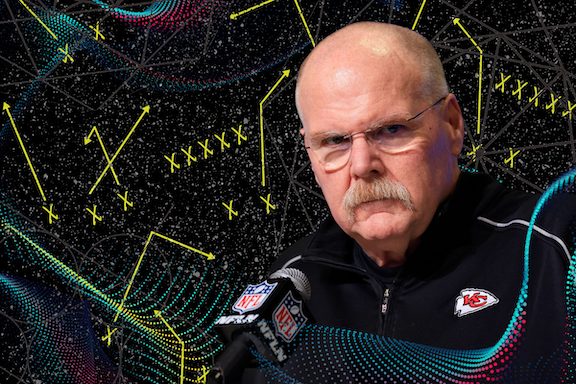
\includegraphics[width=0.5\textwidth,height=\textheight]{img/andy.png}
\caption{Forward by Andy `The Chef' Reid}
\end{figure}

This is America, gentlemen, you play to win. If it is ping-pong or a hot
dog eating contest, you play to win. That is how you go about this
business we call Dynasty Fantasy Football. It is all about getting that
sweet, sweet taste of victory.

Maybe you won last year. Maybe you didn't deserve to, either. Doesn't
matter to me. If you like chocolate cake and you eat a piece, and then
you have one dangling in front of your face, you're going to want to eat
that too. And hungry dogs run faster.

This isn't gonna be easy but its gonna be worth it. Building a dynasty
team, cultivating these players, it's a lot like a great burger. It's
hard, I mean, you have to execute that thing just the right way. You
have to get it to where it's perfect and juicy when you cut it open but
not raw. Then add a nice slice of a Vidalia onion, some mayo, ketchup, a
little squirt of mustard - but not too much - pickles, lettuce and
tomato and baby I'm ready to roll.

To put all that together and make it perfect, there's some time
involved. That's where the real work comes in. You practice, you get it
right, you perfect your craft and then when you finally bite into it,
hoo boy, that's ecstasy right there. So, that's why we play. In my book,
there isn't a real man alive who doesn't love a good hamburger and a
clean hit of ecstasy. Call me old fashioned.

There's a lot of ways to win this league. In some ways you want to keep
the roster young. And at the same time you need those veterans who make
you feel older. That's a delicate blend, not unlike sweet and sour pork.

So go attack this thing, boys. Attack it like I went after a few Chile
Rellenos the other night. Because if you get that trophy, it's a special
feeling, man. It means it all paid off. It'll mean something to you
forever. When you sit back and look at that dick-shaped hunk of metal
with your name on it, it brings a smile to your face. It's like a
Snickers in the freezer, right? It's treasured.

\begin{figure}
\centering
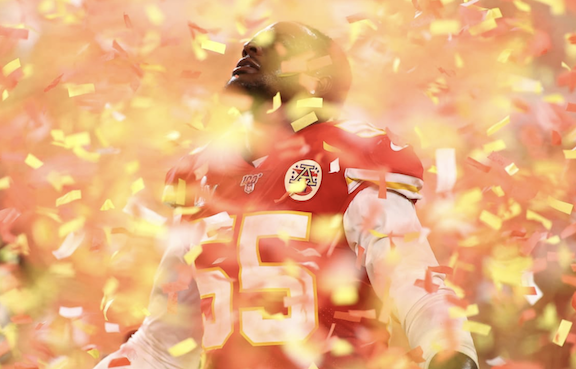
\includegraphics{img/confetti.png}
\caption{The Goal}
\end{figure}

\newpage

\hypertarget{the-results}{%
\subsection{The Results}\label{the-results}}

\hypertarget{final-standings}{%
\subsubsection{Final Standings}\label{final-standings}}

\textbf{All-Time Dynasty Standings \& 2022 Final Regular Season
Standings}

\begin{figure}

{\centering 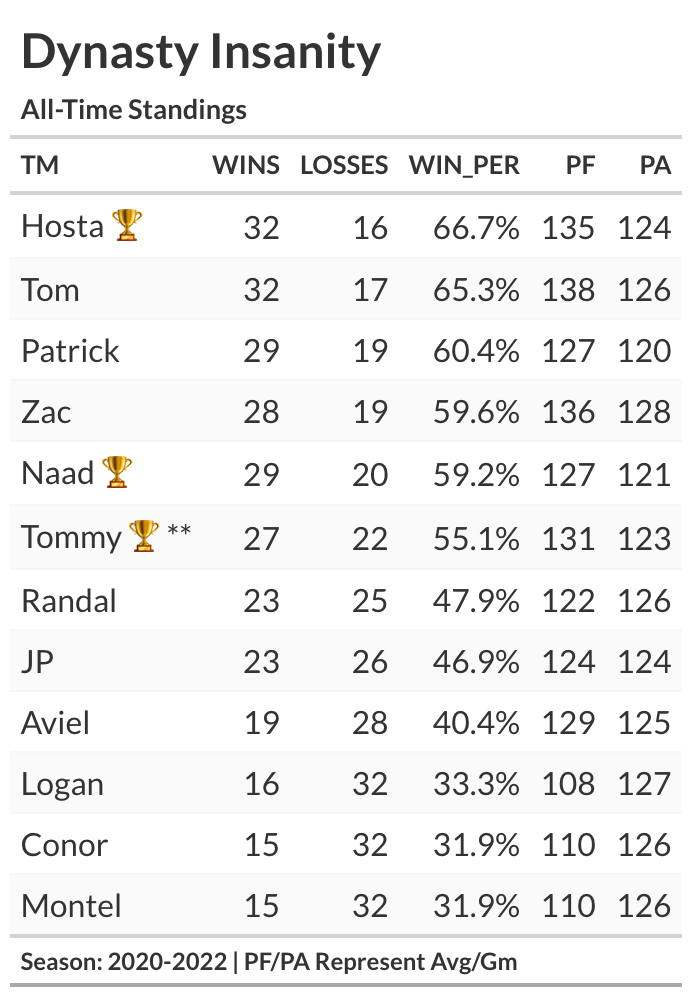
\includegraphics[width=0.49\linewidth,height=0.49\textheight]{output/history/all_time_standings} 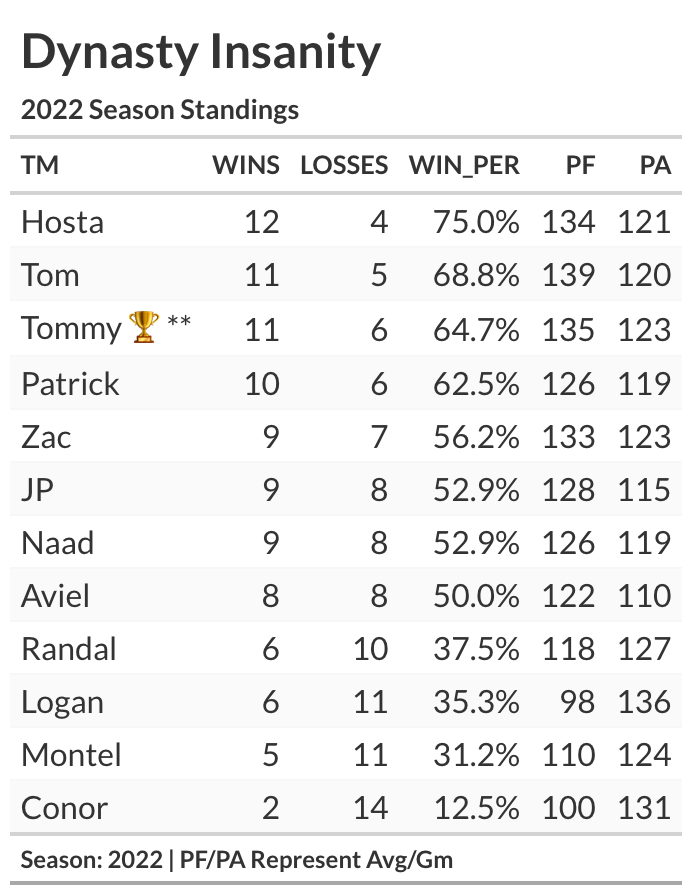
\includegraphics[width=0.49\linewidth,height=0.49\textheight]{output/history/2022_standings} 

}

\caption{Standings}\label{fig:unnamed-chunk-2}
\end{figure}
\newpage

\textbf{2021 \& 2020 Final Regular Season Standings}

\begin{figure}

{\centering 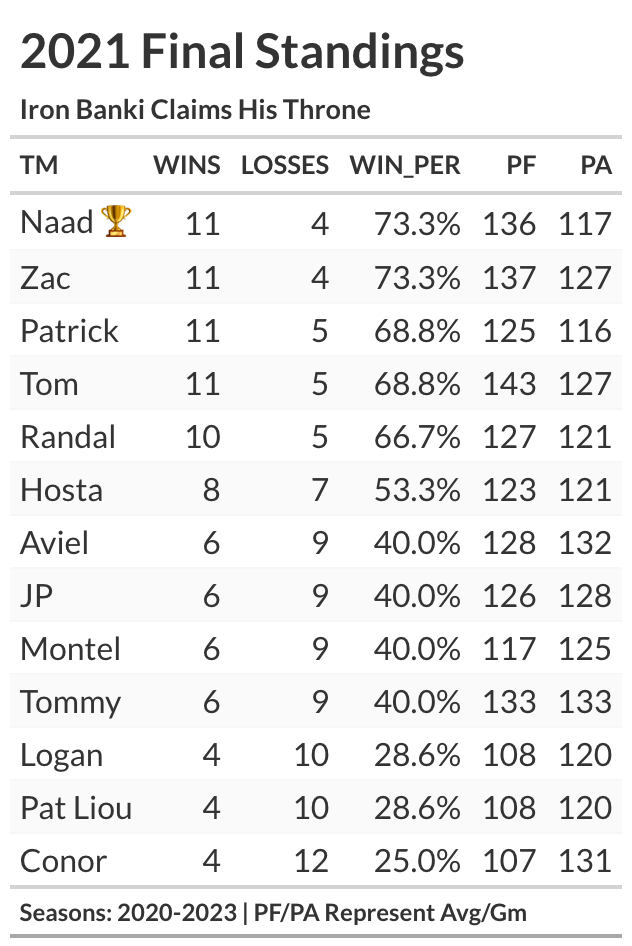
\includegraphics[width=0.5\linewidth,height=0.5\textheight]{output/history/2021_standings} 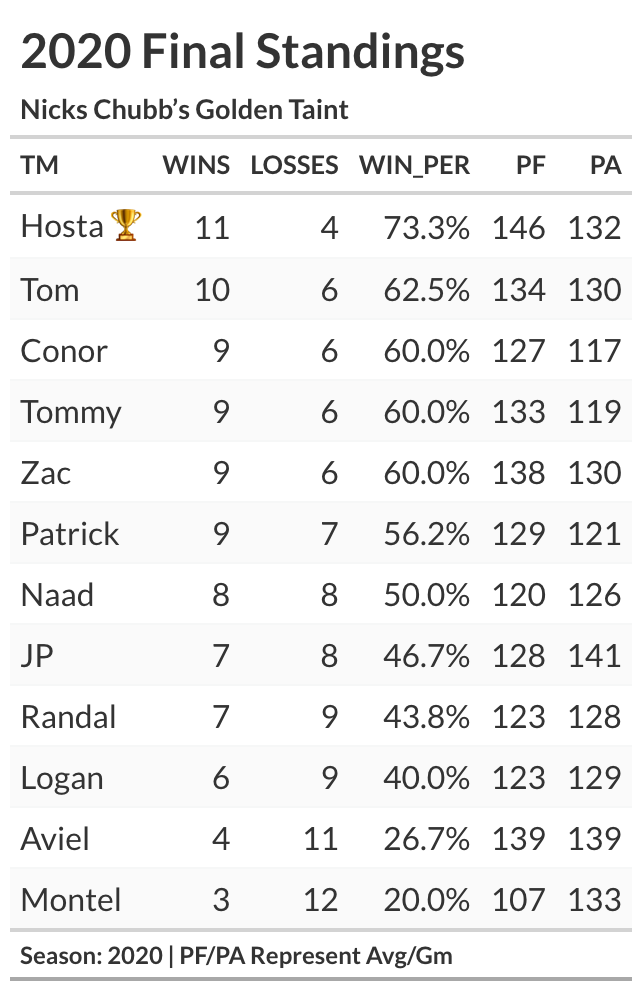
\includegraphics[width=0.5\linewidth,height=0.5\textheight]{output/history/2020_standings} 

}

\caption{Standings}\label{fig:unnamed-chunk-3}
\end{figure}
\newpage

\hypertarget{notable-matchups}{%
\subsubsection{Notable Matchups}\label{notable-matchups}}

\textbf{Blowouts and Nail Biters}

\begin{figure}

{\centering 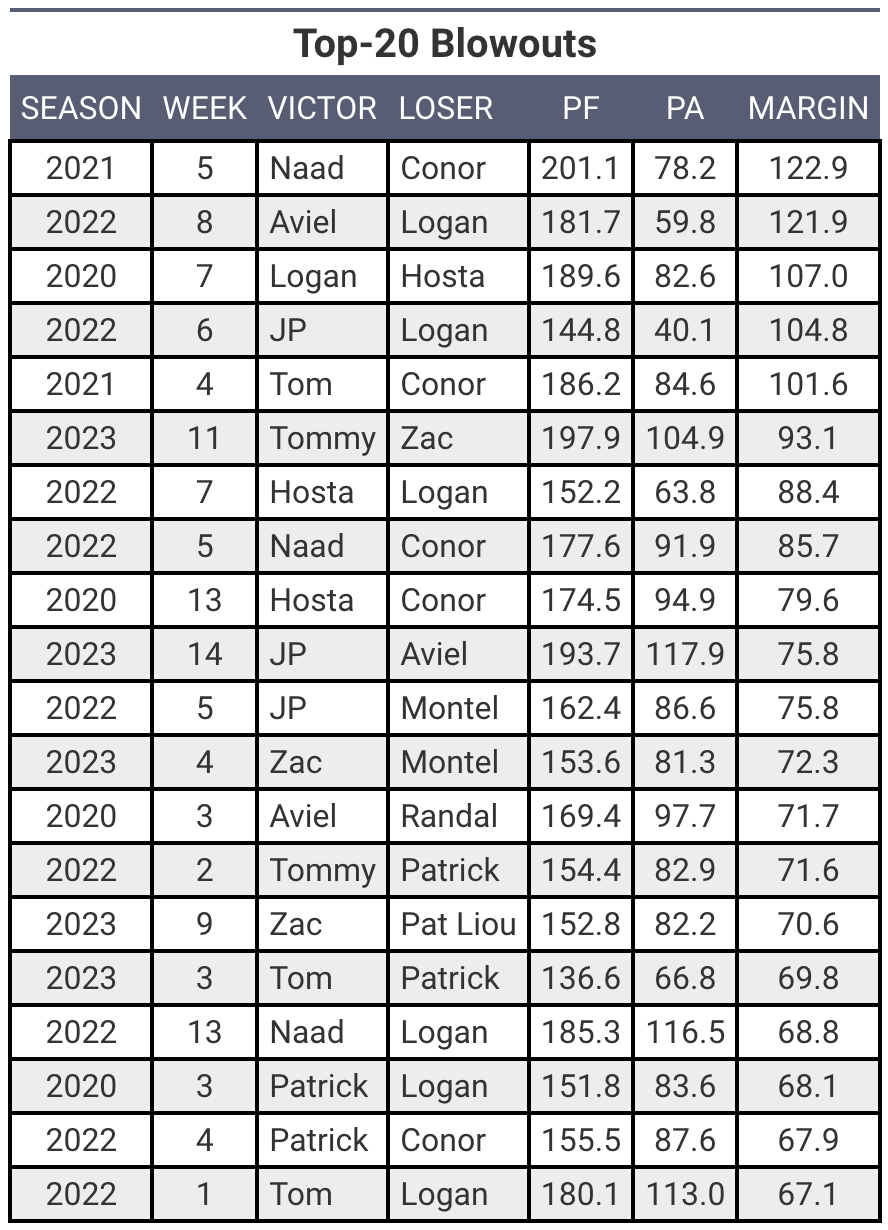
\includegraphics[width=0.5\linewidth,height=0.5\textheight]{output/history/blowouts} 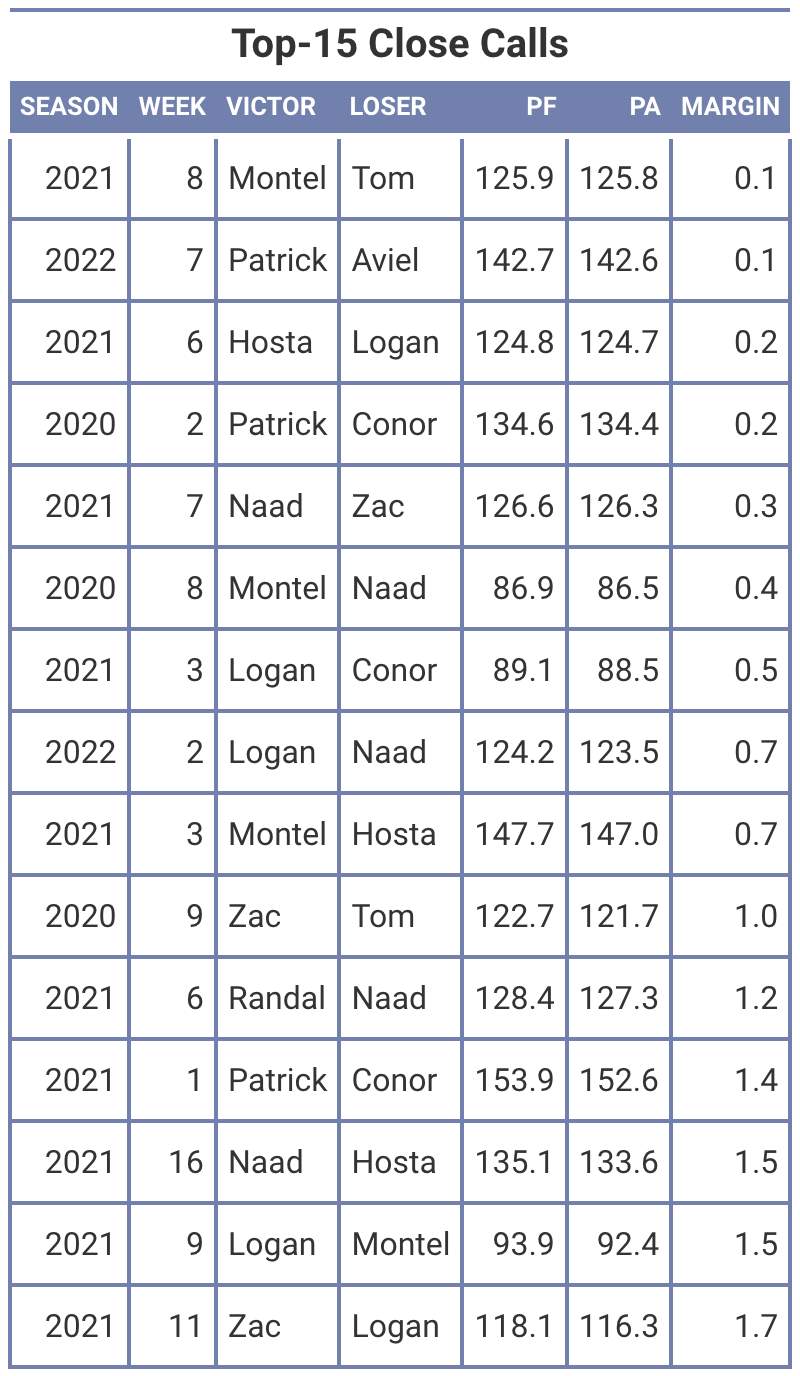
\includegraphics[width=0.5\linewidth,height=0.5\textheight]{output/history/closecalls} 

}

\caption{Just Win, Baby!}\label{fig:unnamed-chunk-4}
\end{figure}

\hypertarget{power-rankings}{%
\subsubsection{Power Rankings}\label{power-rankings}}

\begin{cols}

\begin{col}{0.3\textwidth}
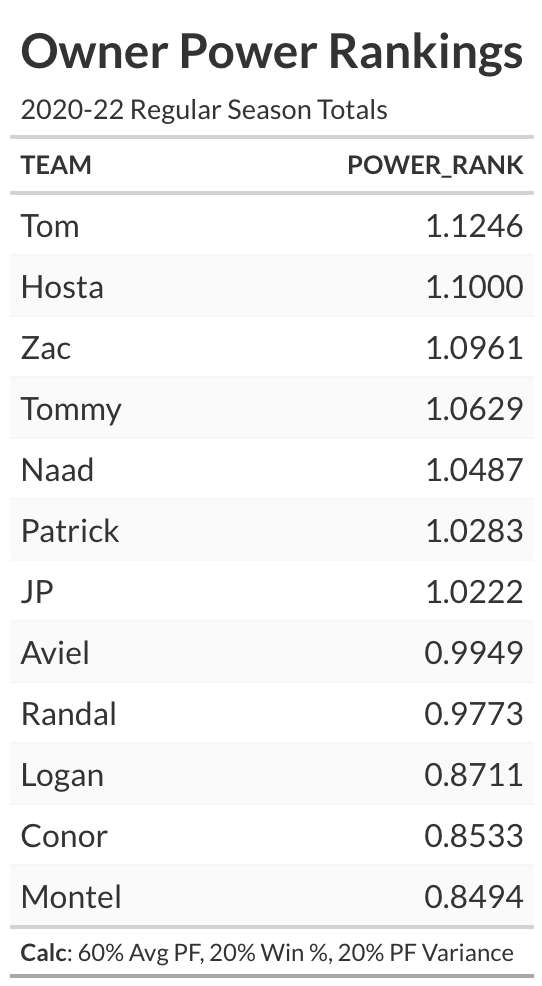
\includegraphics[width=0.7\linewidth]{output/history/all_time_power_rank_standings_owner}
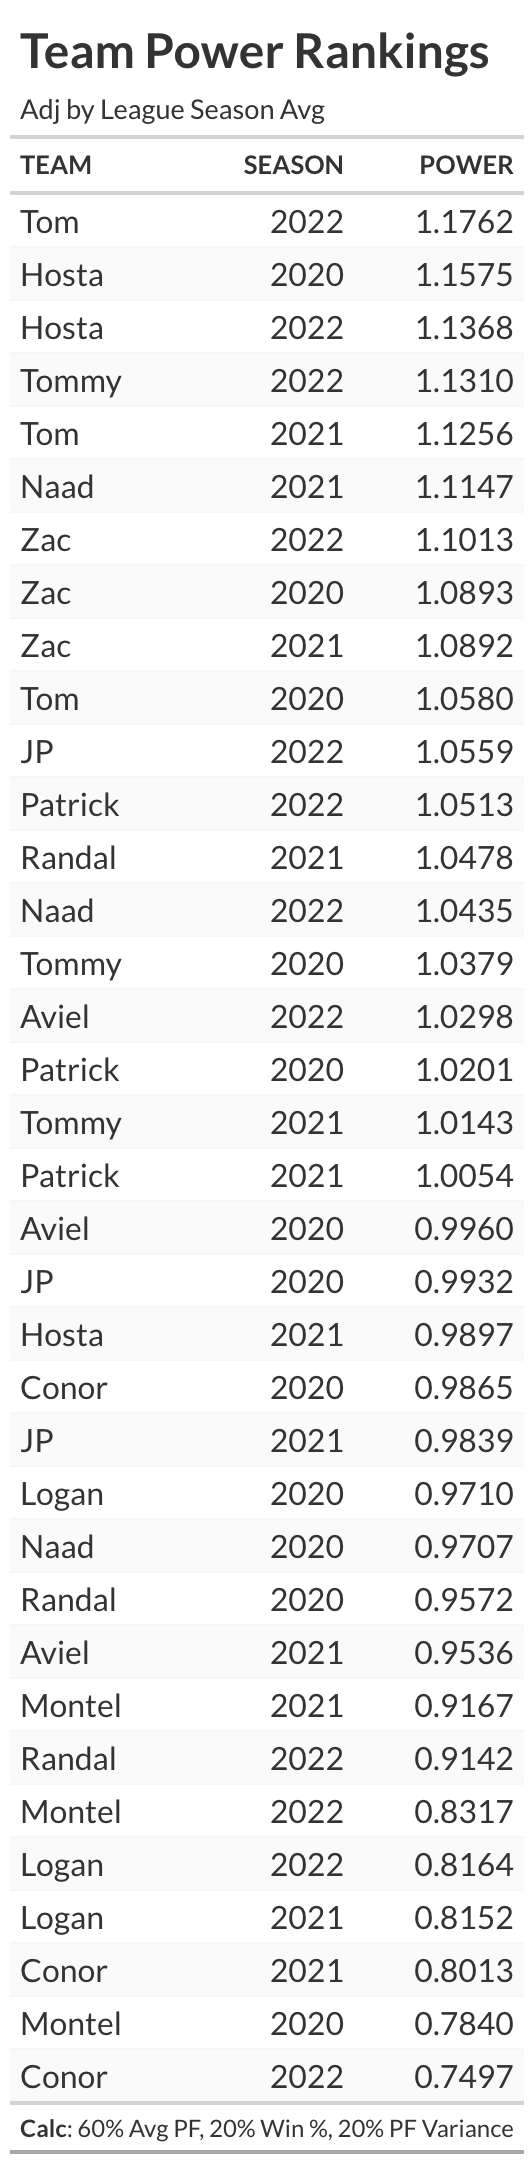
\includegraphics[width=0.7\linewidth]{output/history/all_time_power_rank_standings_yearly}

\end{col}

\begin{col}{0.05\textwidth}
~

\end{col}

\begin{col}{0.65\textwidth}
The figure on the left-hand side shows the \texttt{power\_ranking} data.
Lorem ipsum dolor sit amet, consectetur adipiscing elit, sed do eiusmod
tempor incididunt ut labore et dolore magna aliqua. Ut enim ad minim
veniam, quis nostrud exercitation ullamco laboris nisi ut aliquip ex ea
commodo consequat. Duis aute irure dolor in reprehenderit in voluptate
velit esse cillum dolore eu fugiat nulla pariatur. Lorem ipsum dolor sit
amet, consectetur adipiscing elit, sed do eiusmod tempor incididunt ut
labore et dolore magna aliqua. Ut enim ad minim veniam, quis nostrud
exercitation ullamco laboris nisi ut aliquip ex ea commodo consequat.
Duis aute irure dolor in reprehenderit in voluptate velit esse cillum
dolore eu fugiat nulla pariatur.

Lorem ipsum dolor sit amet, consectetur adipiscing elit, sed do eiusmod
tempor incididunt ut labore et dolore magna aliqua. Ut enim ad minim
veniam, quis nostrud exercitation ullamco laboris nisi ut aliquip ex ea
commodo consequat. Duis aute irure dolor in reprehenderit in voluptate
velit esse cillum dolore eu fugiat nulla pariatur.

\end{col}

\end{cols}

\newpage

\hypertarget{the-franchises}{%
\subsection{The Franchises}\label{the-franchises}}

It's almost Week 1 and these are the final rosters each Franchise has
selected, by choice or not, to take the field.

Anyone of you can build plausible-sounding, `fact-based' narratives that
attempt to explain why your roster is taking home the trophy. Only time
will tell.

Hopefully, 2023 doesn't require a tragic, near-death on live TV to
determine its outcome. In a perfect world, it won't end with a tainted,
asterisk-bound title. I think that's something we can all agree on -
unlike saying, ``Congrats, Tommy Tsao!''

With that - on to 2023 and previewing each franchise's 2023 roster,
strengths, weaknesses, historical results and rivals. A Dynasty version
of Why Your Team Sucks but, unlike Deadspin's review of the NFL, most of
your guy's rosters are genuine, Oakland-level dogshit.

\emph{To preview each team, the following information is aggregated:}

\begin{enumerate}
\def\labelenumi{\arabic{enumi}.}
\item
  2023 Pre-Draft Roster (Including Various Rankings)
\item
  2022 Final Roster (Ranked by Fantasy Points Scored in Line-Up)
\item
  2022 Final Schedule Win/Loss
\item
  Career Head to Head Records vs League Opponents (All-Time)
\end{enumerate}

\emph{Notes on Methodology:}

\begin{enumerate}
\def\labelenumi{\arabic{enumi}.}
\item
  Ranking, Tier, and ECR Sourced via \textbf{FantasyPros}
\item
  Position Rank and Career Value Sourced via \textbf{DynastyProcess.com}
\item
  Lifetime Value Sourced via \textbf{PlayerProfiler}
\item
  Bench Players Limited to \textbf{Top 10 by FantasyPros Ranking}
\end{enumerate}

\newpage

\hypertarget{alanasty}{%
\subsubsection{Alanasty}\label{alanasty}}

\textbf{2023 Proj. \& 2022 Final Rosters}

\begin{figure}

{\centering 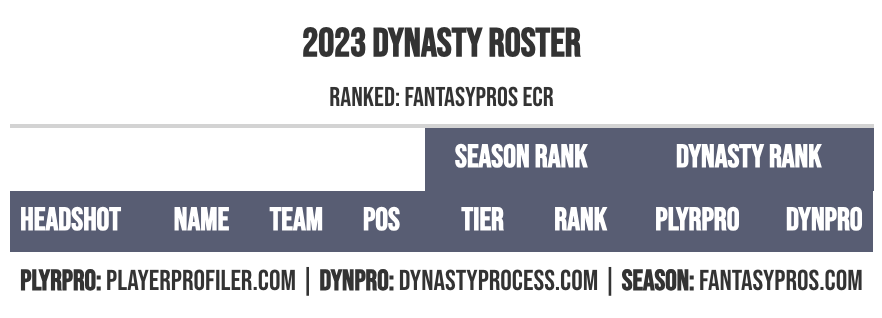
\includegraphics[width=0.7\linewidth,height=0.7\textheight]{output/2023/dynasty_roster_Alanasty} 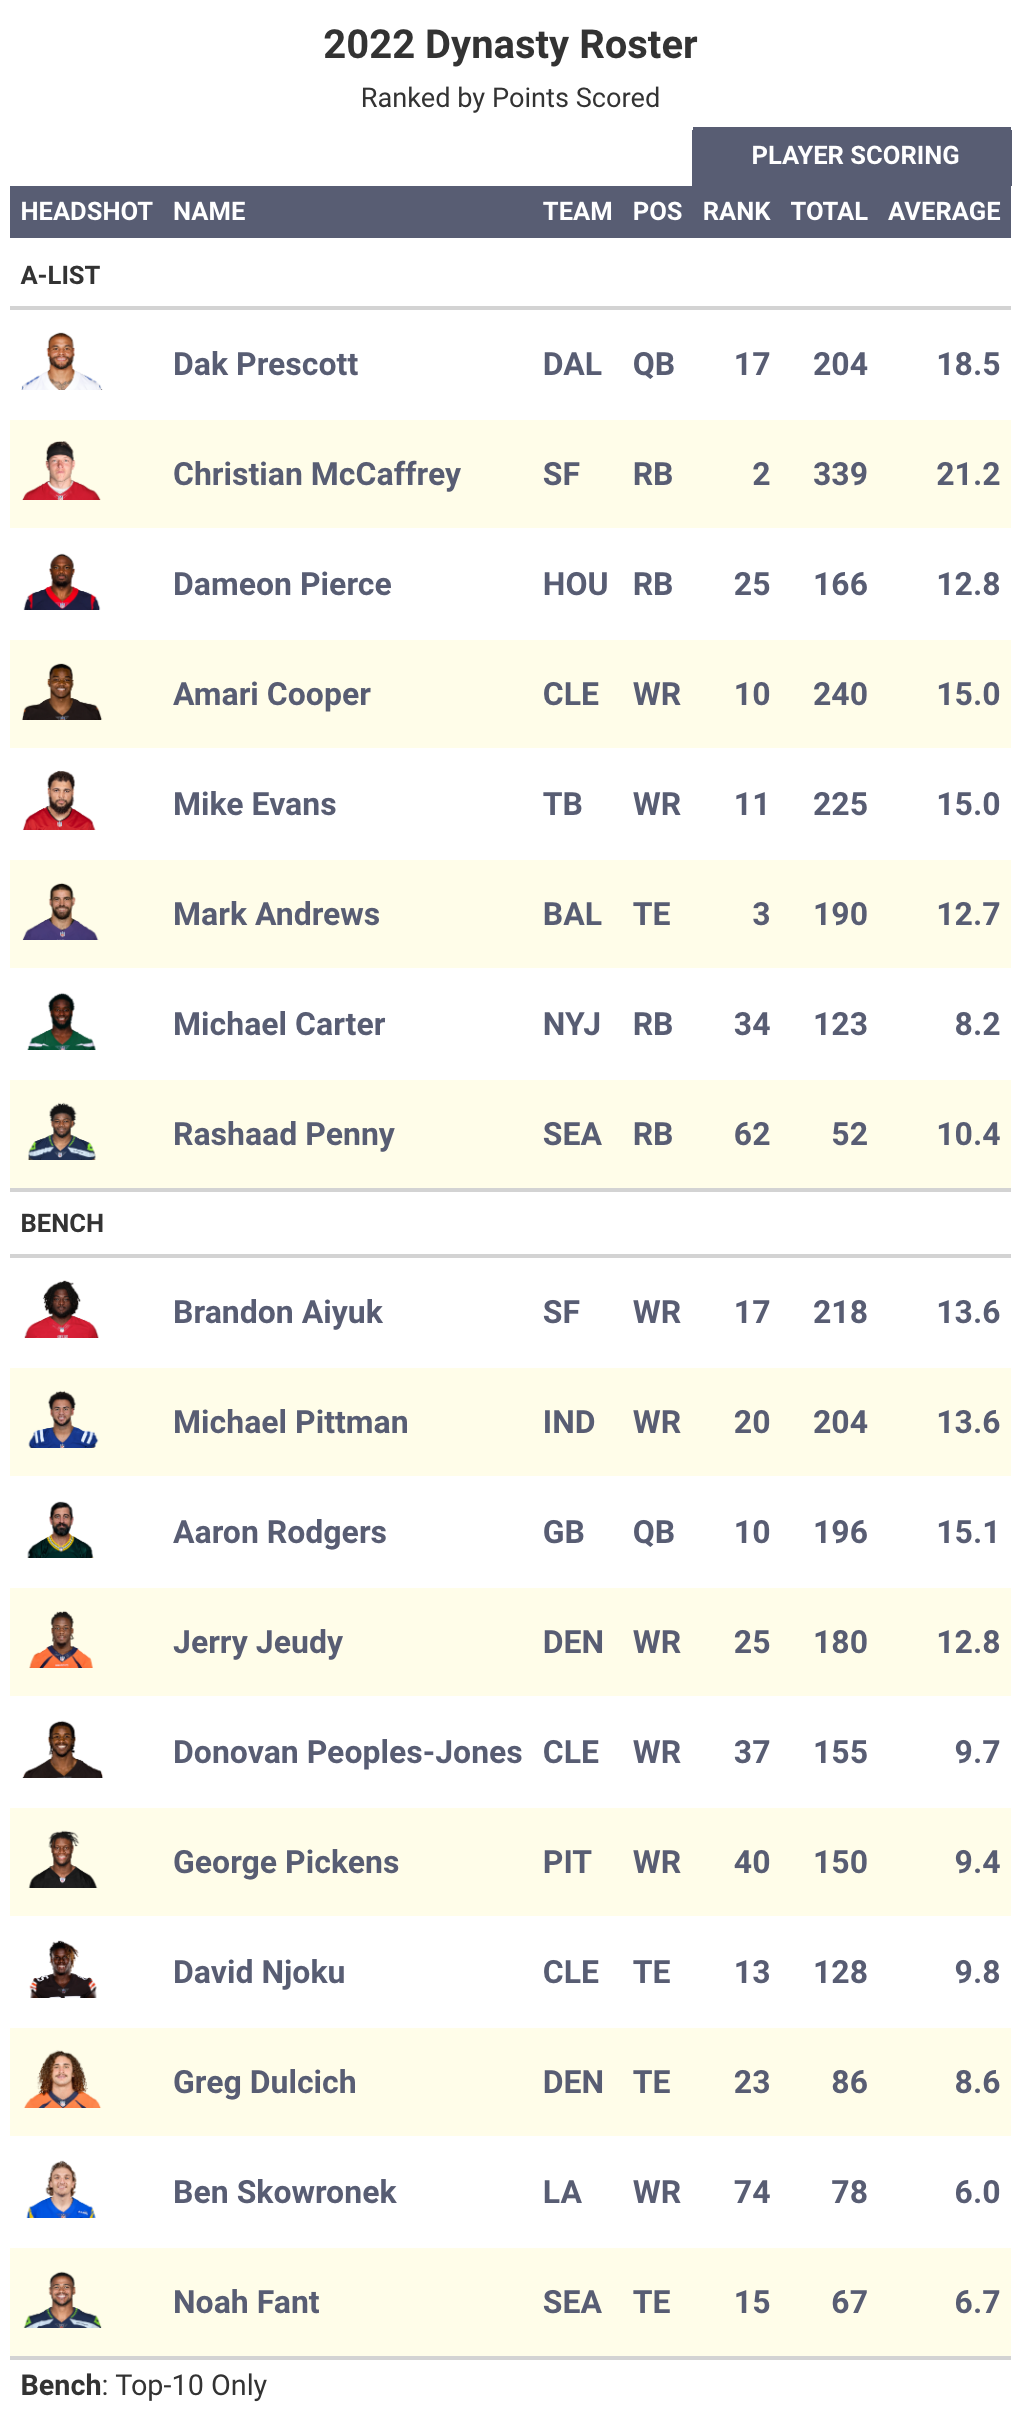
\includegraphics[width=0.7\linewidth,height=0.7\textheight]{output/2022/dynasty_roster_Alanasty} 

}

\caption{The Ballers}\label{fig:unnamed-chunk-5}
\end{figure}
\newpage

\textbf{2022 Schedule \& Career Head to Head}

\begin{figure}

{\centering 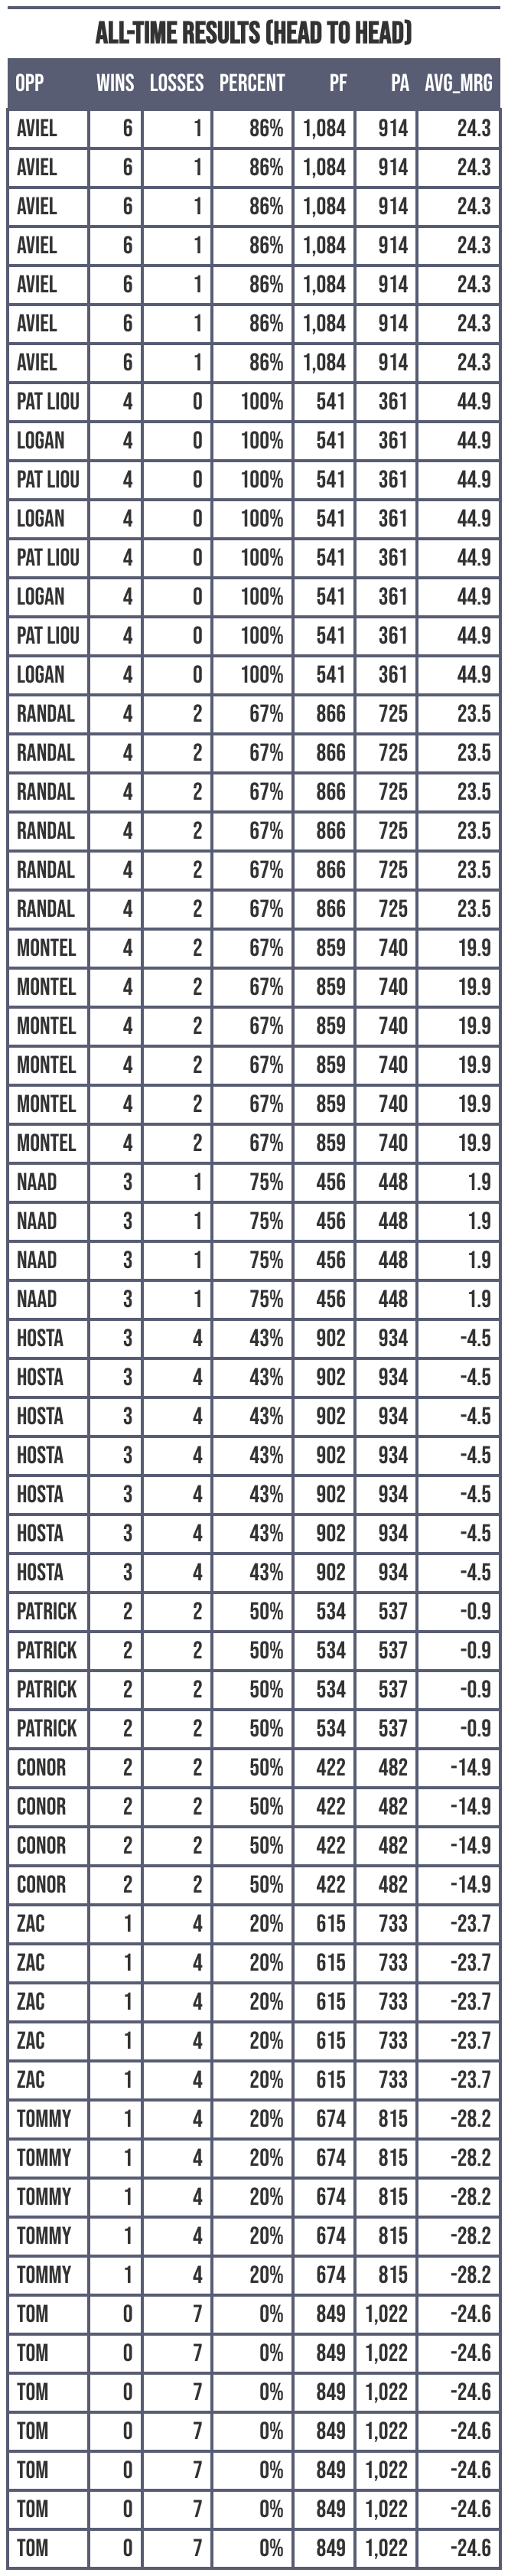
\includegraphics[width=0.48\linewidth,height=0.48\textheight]{output/headtohead/JP_head_to_head} 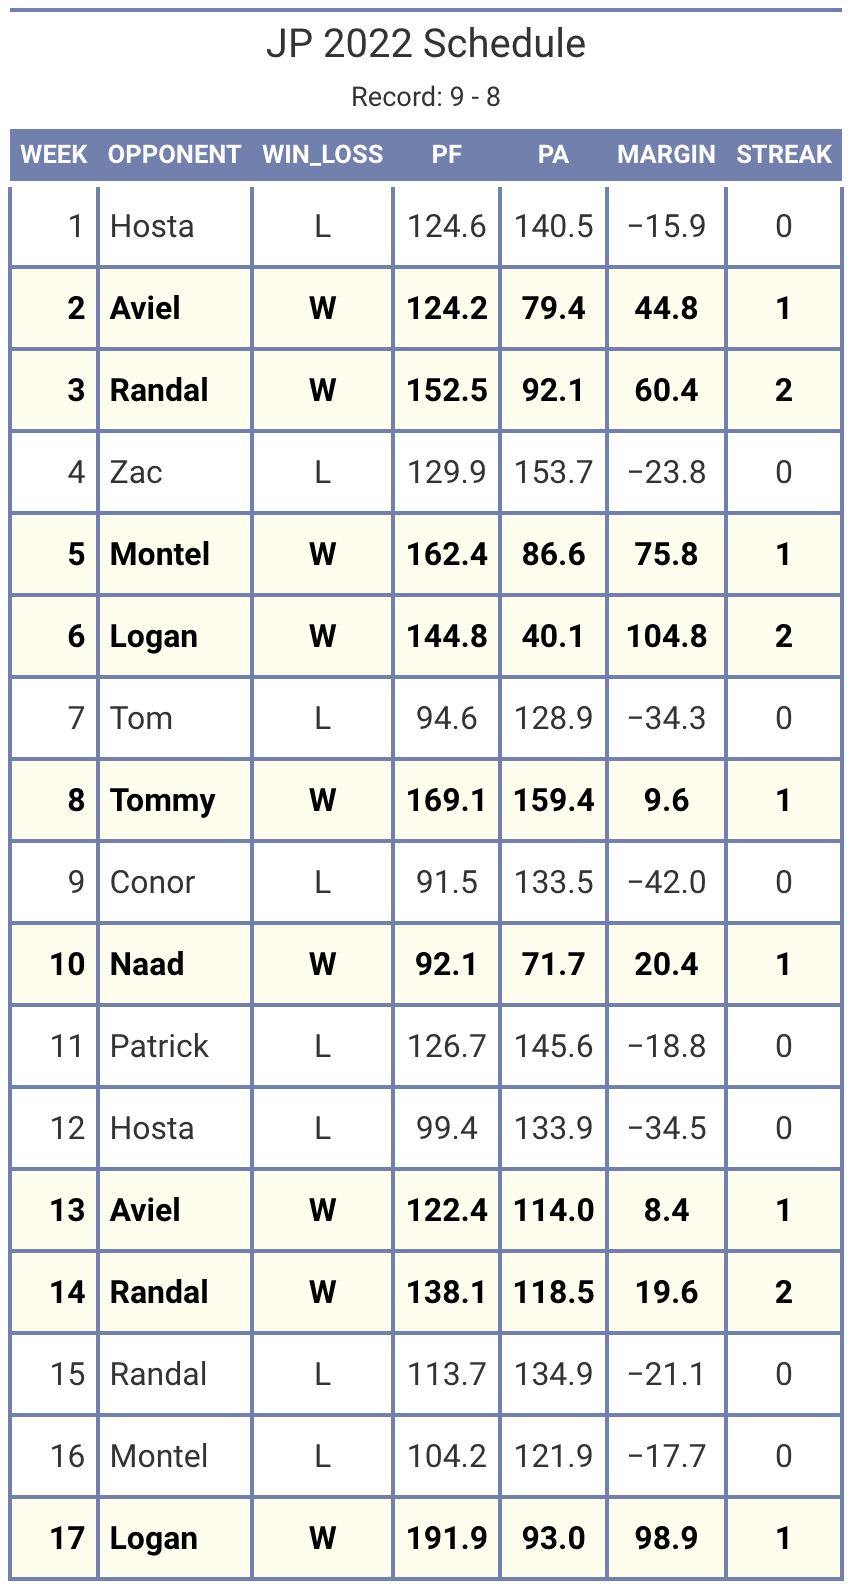
\includegraphics[width=0.48\linewidth,height=0.48\textheight]{output/py_schedule/season_results_JP} 

}

\caption{The Outcomes}\label{fig:unnamed-chunk-6}
\end{figure}
\newpage

\hypertarget{the-iron-banki}{%
\subsubsection{The Iron Banki}\label{the-iron-banki}}

\textbf{2023 Proj. \& 2022 Final Rosters}

\begin{figure}

{\centering \includegraphics[width=0.7\linewidth,height=0.7\textheight]{output/2023/dynasty_roster_Naaderbanki} \includegraphics[width=0.7\linewidth,height=0.7\textheight]{output/2022/dynasty_roster_Naaderbanki} 

}

\caption{The Ballers}\label{fig:unnamed-chunk-7}
\end{figure}
\newpage

\textbf{2022 Schedule \& Career Head to Head}

\begin{figure}

{\centering 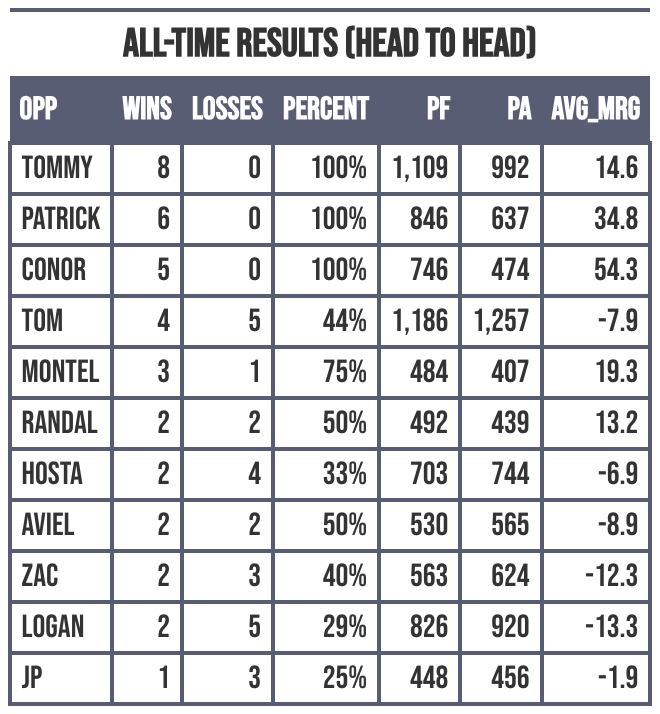
\includegraphics[width=0.48\linewidth,height=0.48\textheight]{output/headtohead/Naad_head_to_head} 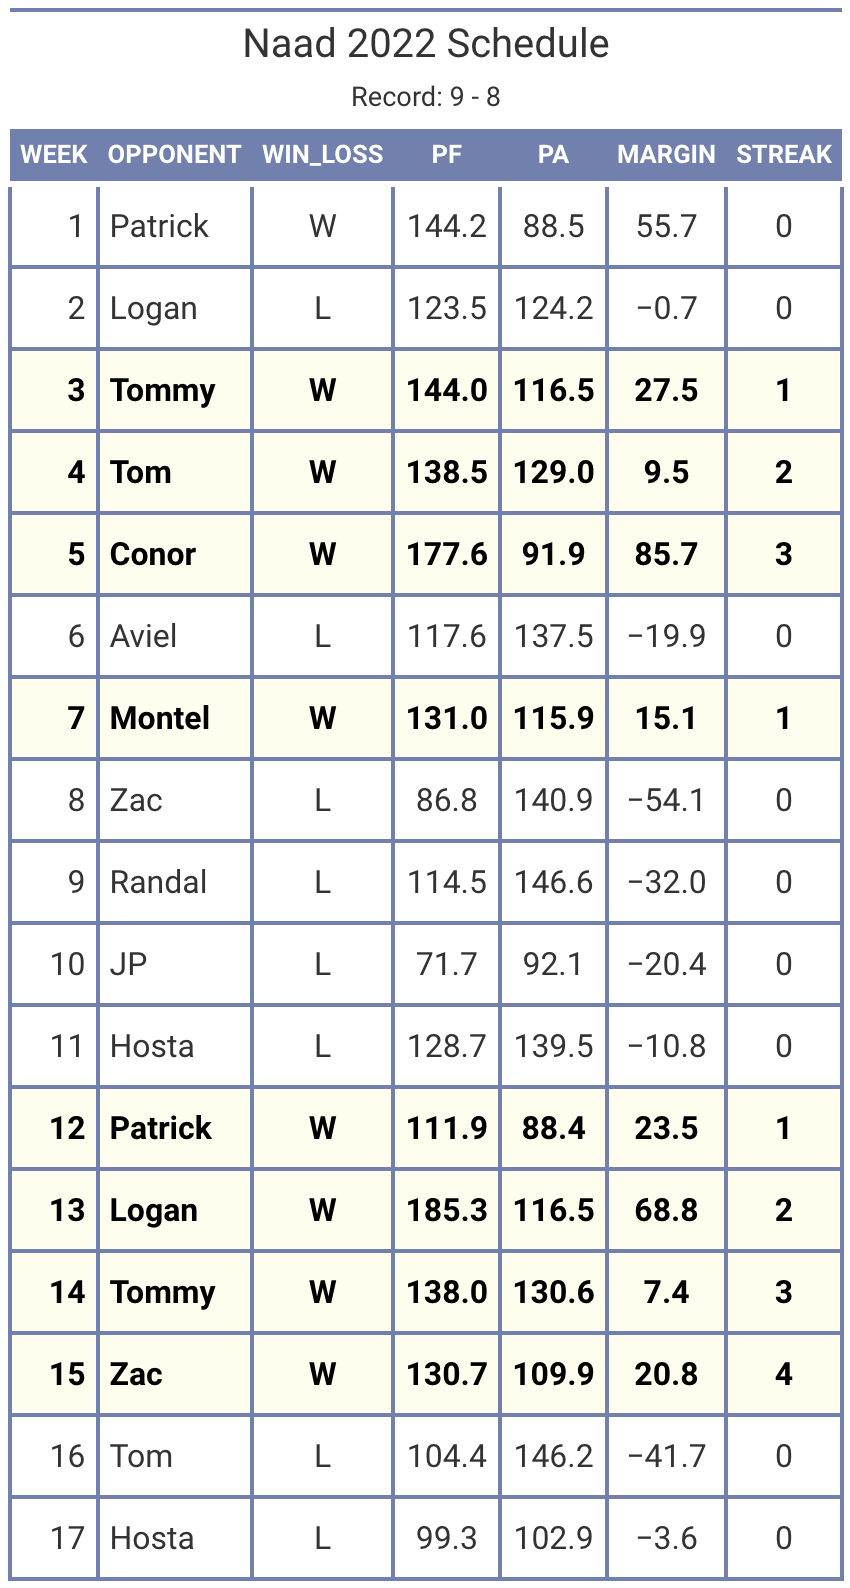
\includegraphics[width=0.48\linewidth,height=0.48\textheight]{output/py_schedule/season_results_Naad} 

}

\caption{The Outcomes}\label{fig:unnamed-chunk-8}
\end{figure}
\newpage

\hypertarget{montels-amen}{%
\subsubsection{Montel's A\$\$men}\label{montels-amen}}

\textbf{2023 Proj. \& 2022 Final Rosters}

\begin{figure}

{\centering \includegraphics[width=0.7\linewidth,height=0.7\textheight]{output/2023/dynasty_roster_Asmontalvo} \includegraphics[width=0.7\linewidth,height=0.7\textheight]{output/2022/dynasty_roster_Asmontalvo} 

}

\caption{The Ballers}\label{fig:unnamed-chunk-9}
\end{figure}
\newpage

\textbf{2022 Schedule \& Career Head to Head}

\begin{figure}

{\centering 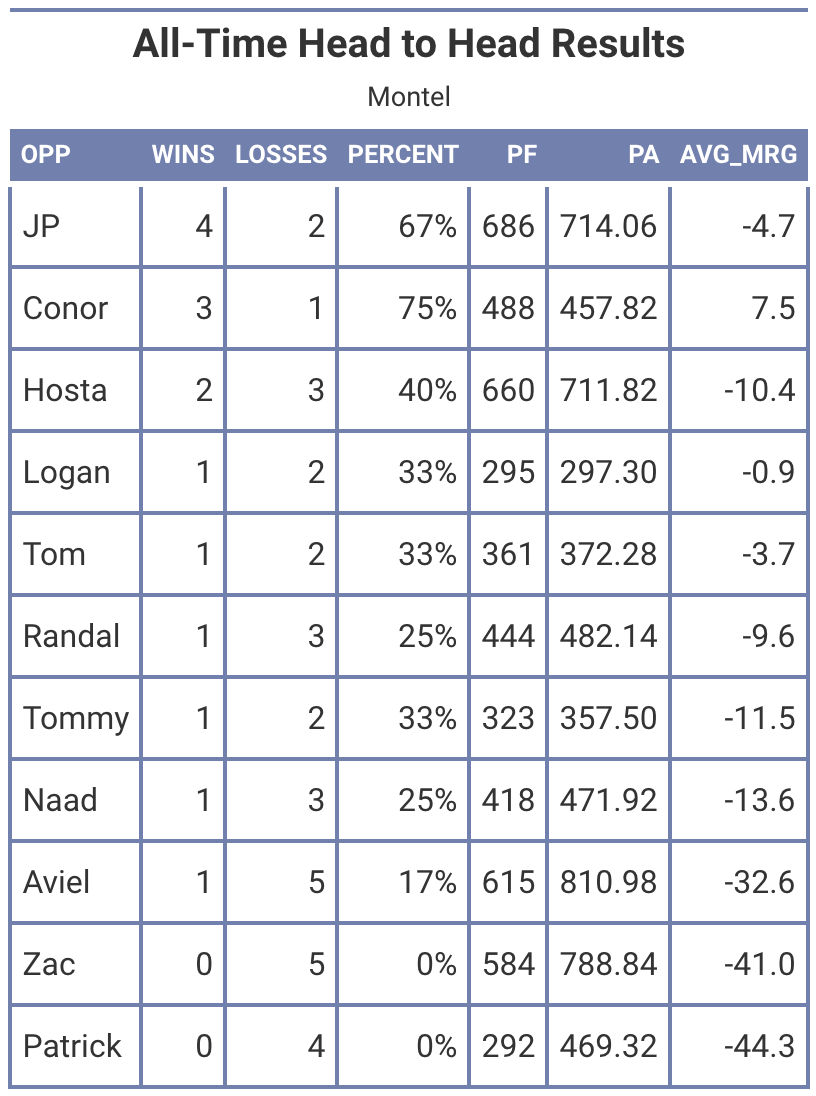
\includegraphics[width=0.48\linewidth,height=0.48\textheight]{output/headtohead/Montel_head_to_head} 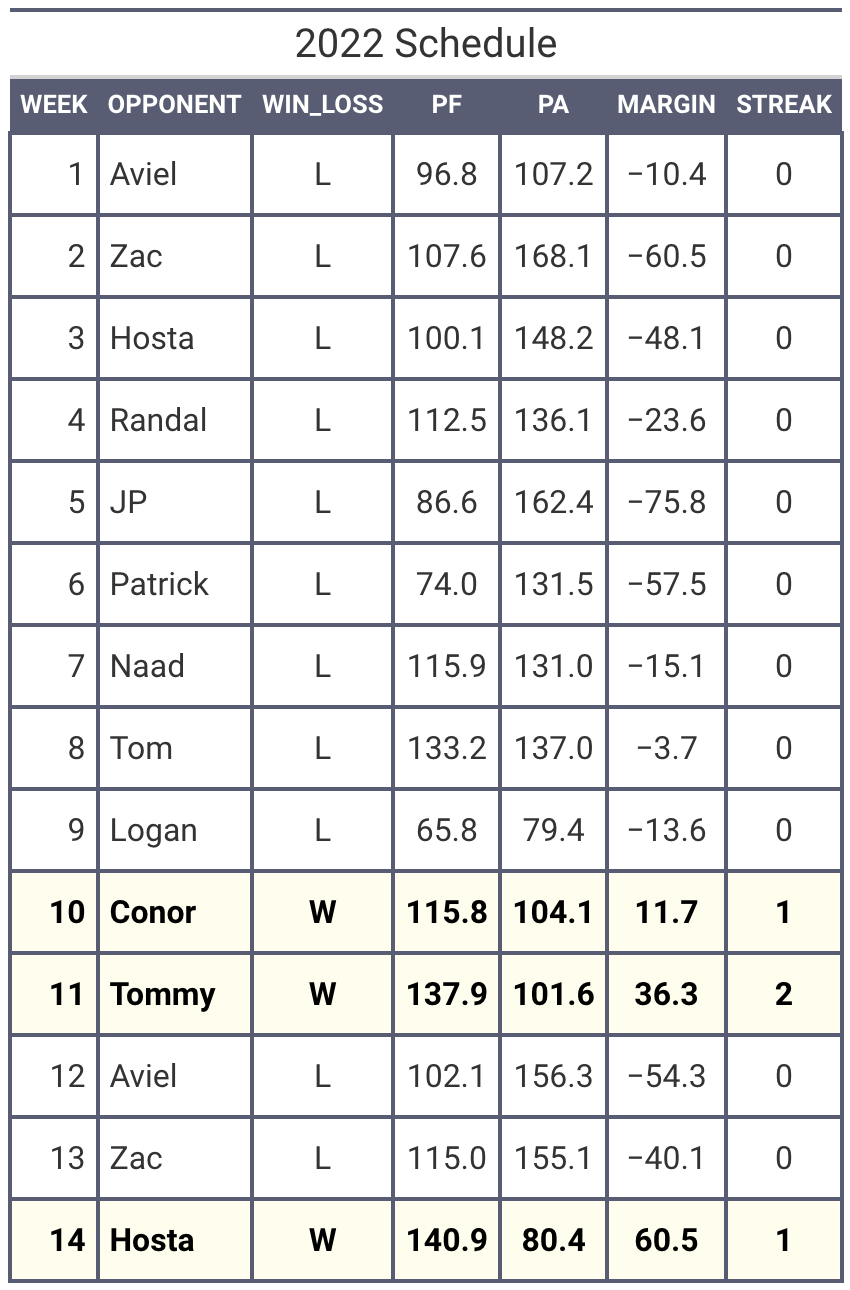
\includegraphics[width=0.48\linewidth,height=0.48\textheight]{output/py_schedule/season_results_Montel} 

}

\caption{The Outcomes}\label{fig:unnamed-chunk-10}
\end{figure}
\newpage

\hypertarget{dick-chubb}{%
\subsubsection{Dick Chubb}\label{dick-chubb}}

\textbf{2023 Proj. \& 2022 Final Rosters}

\begin{figure}

{\centering \includegraphics[width=0.7\linewidth,height=0.7\textheight]{output/2023/dynasty_roster_Nhosta} \includegraphics[width=0.7\linewidth,height=0.7\textheight]{output/2022/dynasty_roster_Nhosta} 

}

\caption{The Ballers}\label{fig:unnamed-chunk-11}
\end{figure}
\newpage

\textbf{2022 Schedule \& Career Head to Head}

\begin{figure}

{\centering 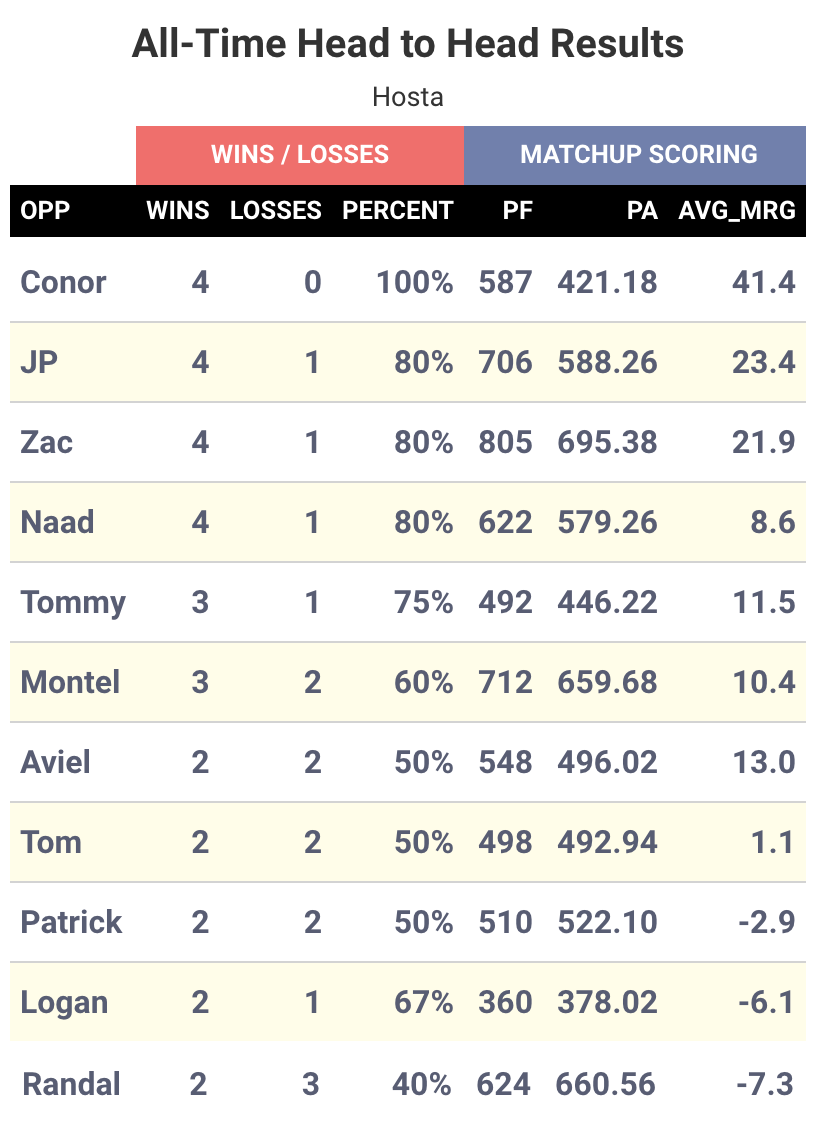
\includegraphics[width=0.48\linewidth,height=0.48\textheight]{output/headtohead/Hosta_head_to_head} 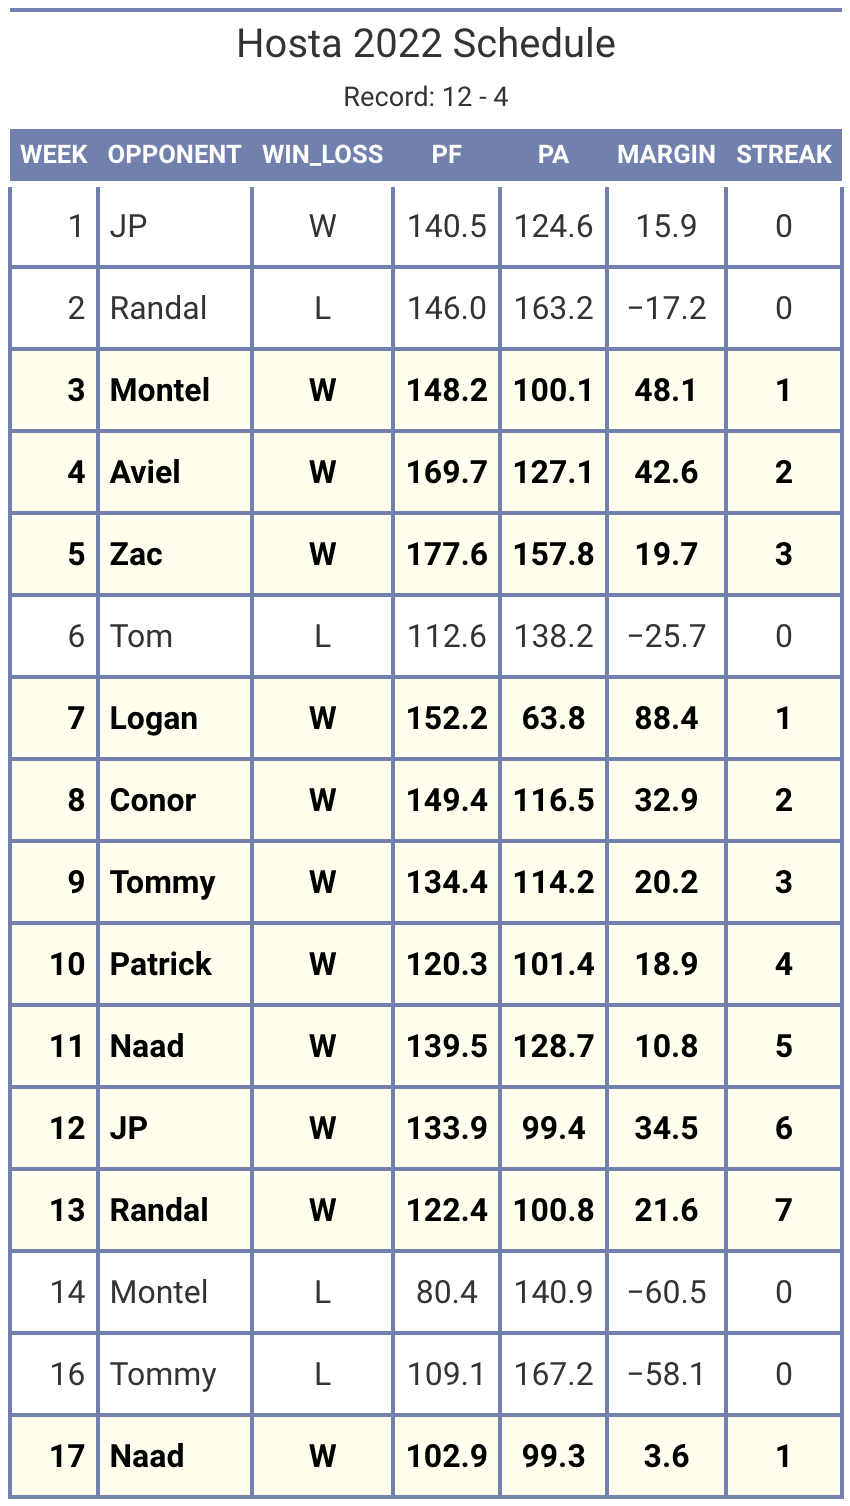
\includegraphics[width=0.48\linewidth,height=0.48\textheight]{output/py_schedule/season_results_Hosta} 

}

\caption{The Outcomes}\label{fig:unnamed-chunk-12}
\end{figure}
\newpage

\hypertarget{andy-reids-briskett}{%
\subsubsection{Andy Reid's Briskett}\label{andy-reids-briskett}}

\textbf{2023 Proj. \& 2022 Final Rosters}

\begin{figure}

{\centering \includegraphics[width=0.7\linewidth,height=0.7\textheight]{output/2023/dynasty_roster_Bellist} \includegraphics[width=0.7\linewidth,height=0.7\textheight]{output/2022/dynasty_roster_Bellist} 

}

\caption{The Ballers}\label{fig:unnamed-chunk-13}
\end{figure}
\newpage

\textbf{2022 Schedule \& Career Head to Head}

\begin{figure}

{\centering 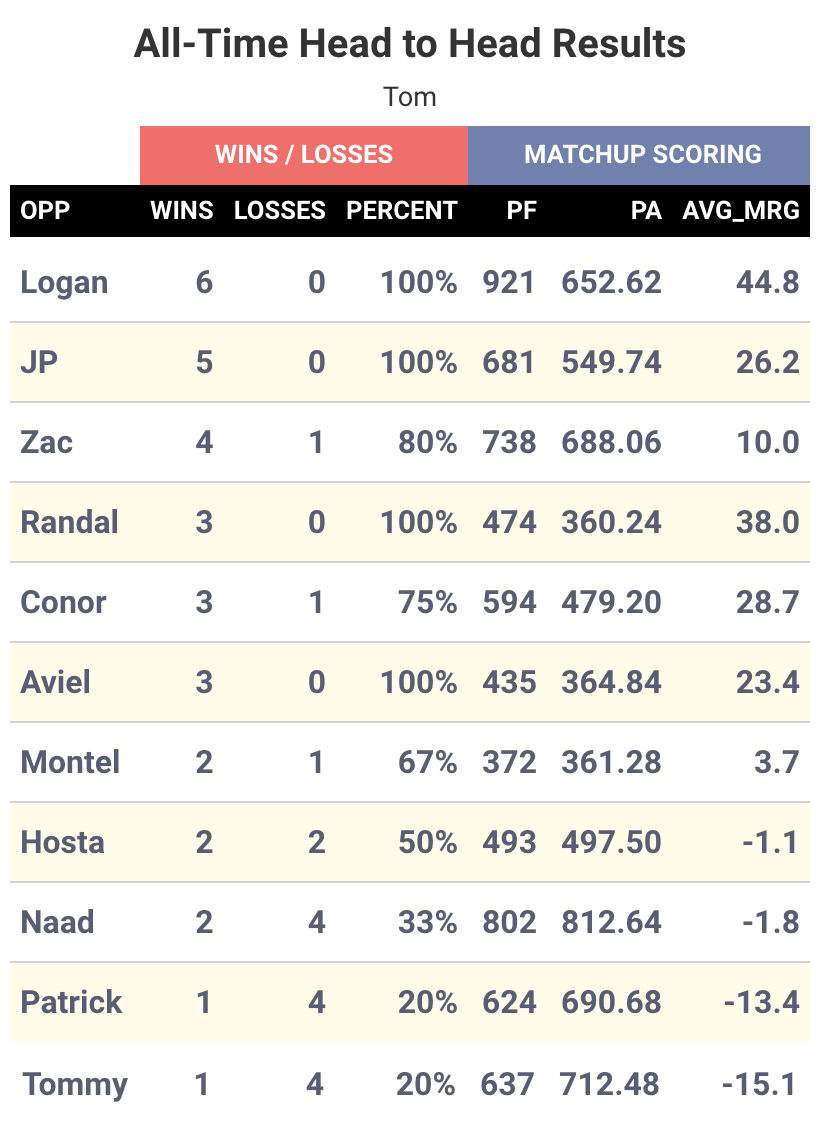
\includegraphics[width=0.48\linewidth,height=0.48\textheight]{output/headtohead/Tom_head_to_head} 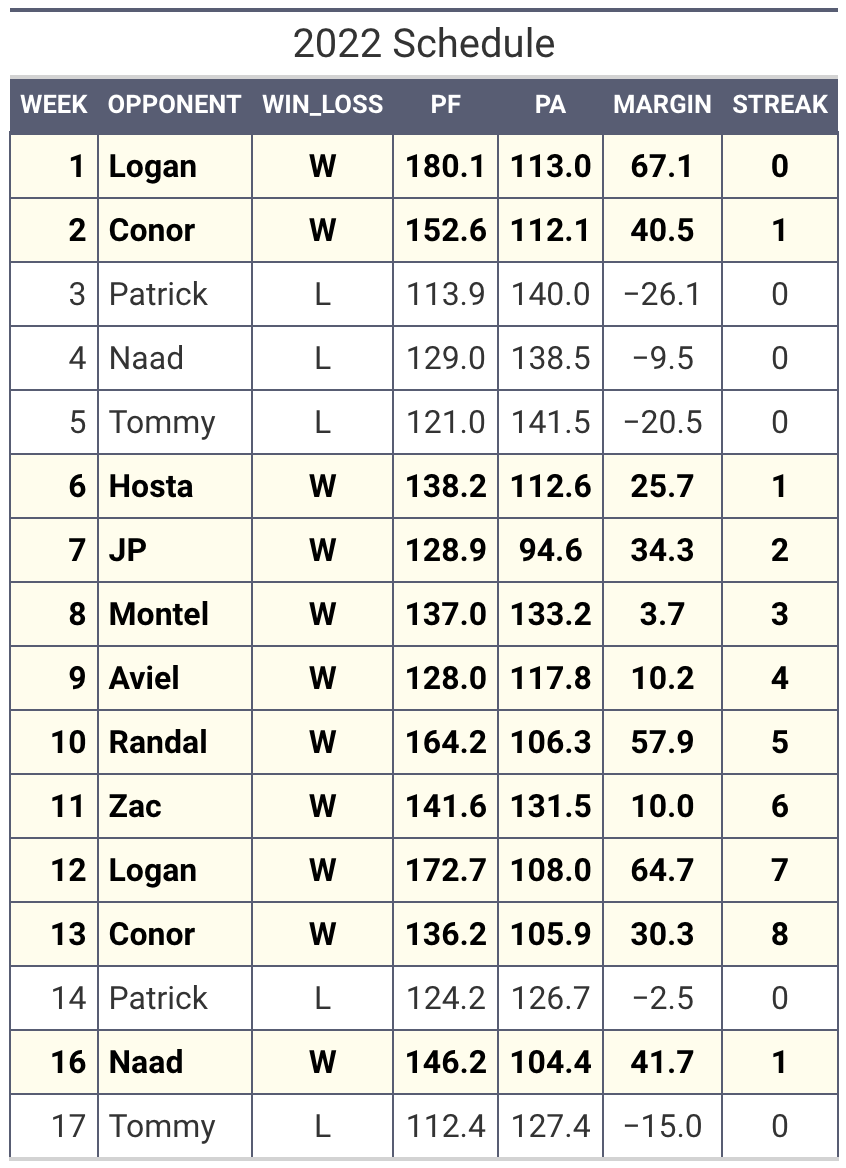
\includegraphics[width=0.48\linewidth,height=0.48\textheight]{output/py_schedule/season_results_Tom} 

}

\caption{The Outcomes}\label{fig:unnamed-chunk-14}
\end{figure}
\newpage

\hypertarget{zac-goffrey}{%
\subsubsection{Zac GOFFrey}\label{zac-goffrey}}

\textbf{2023 Proj. \& 2022 Final Rosters}

\begin{figure}

{\centering \includegraphics[width=0.7\linewidth,height=0.7\textheight]{output/2023/dynasty_roster_Zacgeoffray} \includegraphics[width=0.7\linewidth,height=0.7\textheight]{output/2022/dynasty_roster_Zacgeoffray} 

}

\caption{The Ballers}\label{fig:unnamed-chunk-15}
\end{figure}
\newpage

\textbf{2022 Schedule \& Career Head to Head}

\begin{figure}

{\centering 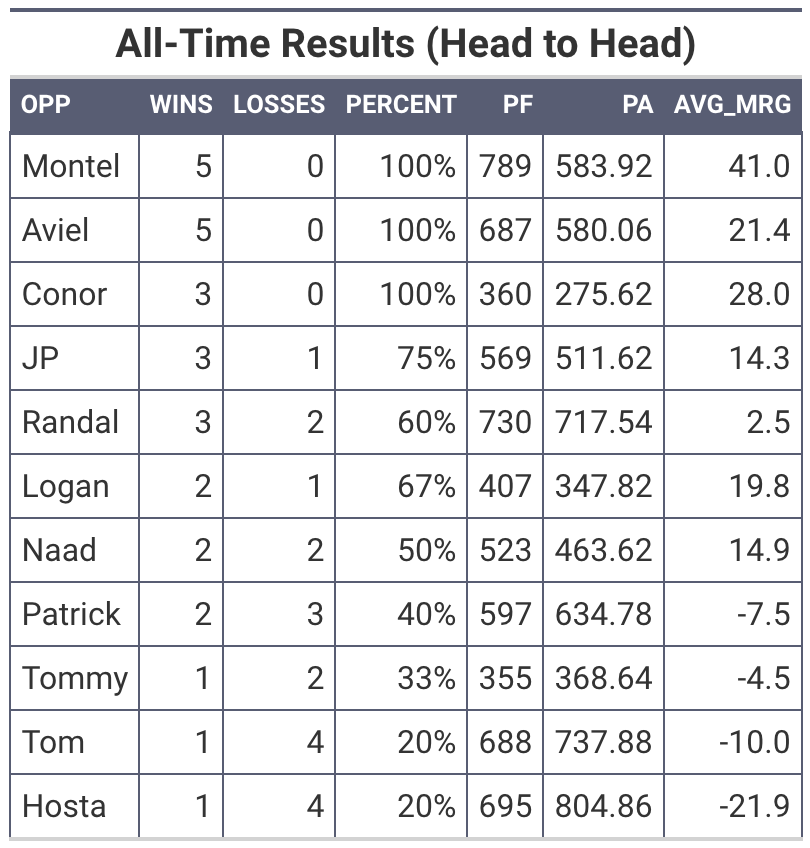
\includegraphics[width=0.48\linewidth,height=0.48\textheight]{output/headtohead/Zac_head_to_head} 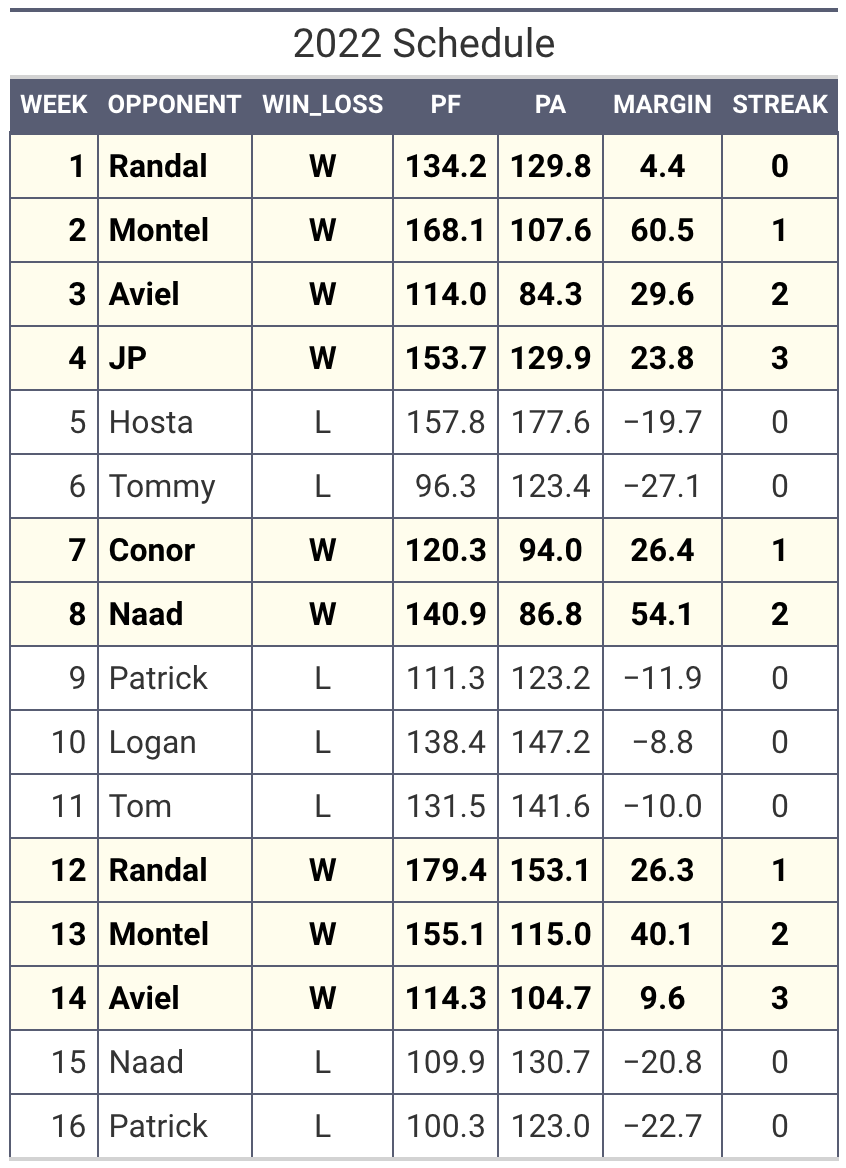
\includegraphics[width=0.48\linewidth,height=0.48\textheight]{output/py_schedule/season_results_Zac} 

}

\caption{The Outcomes}\label{fig:unnamed-chunk-16}
\end{figure}
\newpage

\hypertarget{john-wick-m.d.}{%
\subsubsection{John Wick, M.D.}\label{john-wick-m.d.}}

\textbf{2023 Proj. \& 2022 Final Rosters}

\begin{figure}

{\centering \includegraphics[width=0.7\linewidth,height=0.7\textheight]{output/2023/dynasty_roster_Johnwickmd} \includegraphics[width=0.7\linewidth,height=0.7\textheight]{output/2022/dynasty_roster_Johnwickmd} 

}

\caption{The Ballers}\label{fig:unnamed-chunk-17}
\end{figure}
\newpage

\textbf{2022 Schedule \& Career Head to Head}

\begin{figure}

{\centering 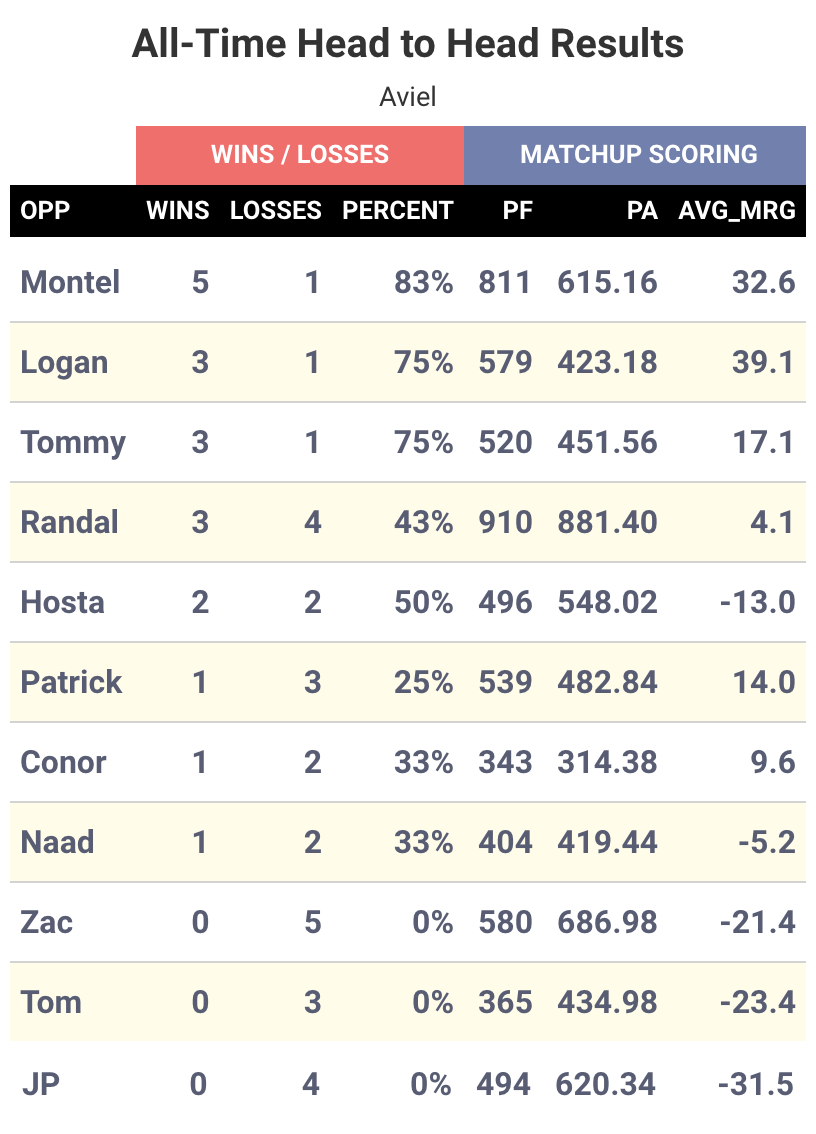
\includegraphics[width=0.48\linewidth,height=0.48\textheight]{output/headtohead/Aviel_head_to_head} 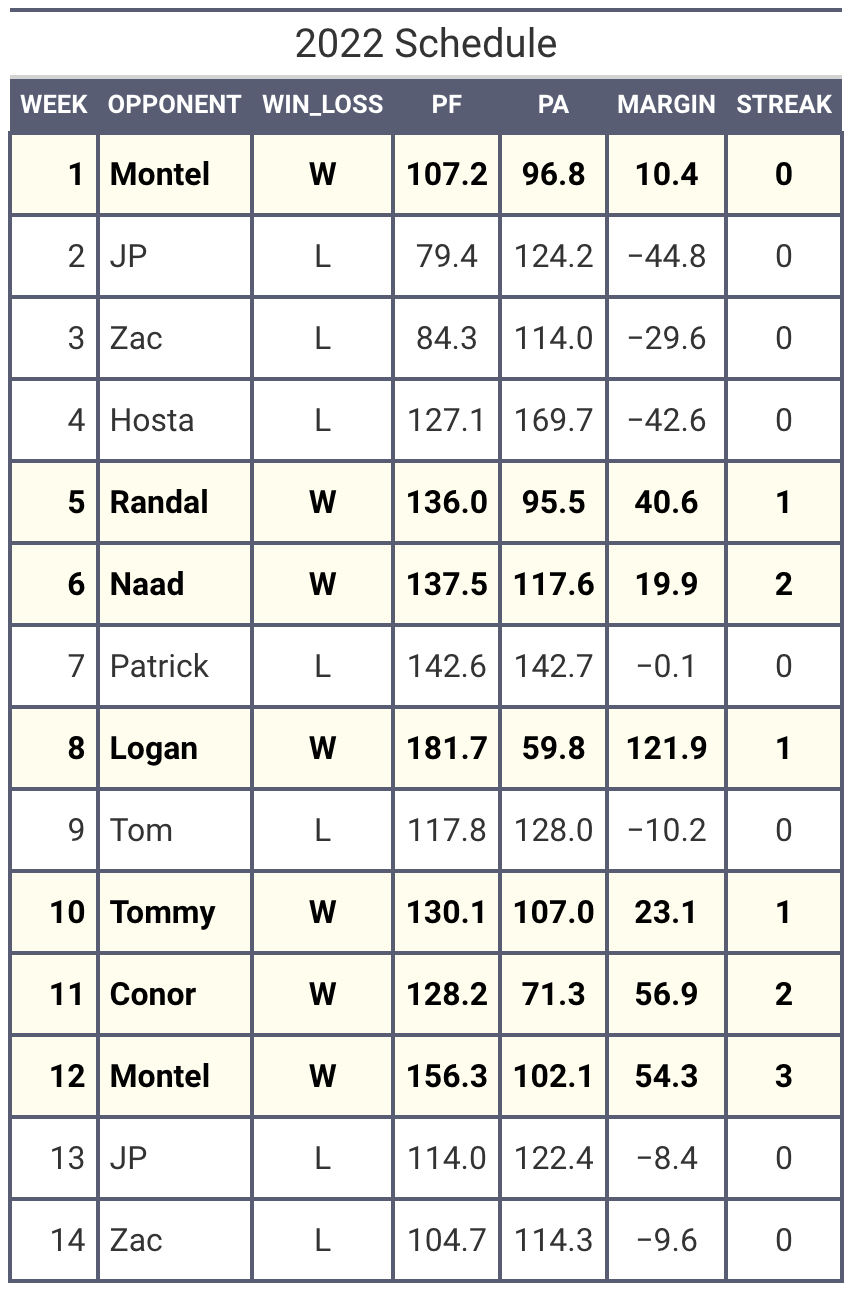
\includegraphics[width=0.48\linewidth,height=0.48\textheight]{output/py_schedule/season_results_Aviel} 

}

\caption{The Outcomes}\label{fig:unnamed-chunk-18}
\end{figure}
\newpage

\hypertarget{conor}{%
\subsubsection{Conor}\label{conor}}

\textbf{2023 Proj. \& 2022 Final Rosters}

\begin{figure}

{\centering \includegraphics[width=0.7\linewidth,height=0.7\textheight]{output/2023/dynasty_roster_Cpmadden1} \includegraphics[width=0.7\linewidth,height=0.7\textheight]{output/2022/dynasty_roster_Cpmadden1} 

}

\caption{The Ballers}\label{fig:unnamed-chunk-19}
\end{figure}
\newpage

\textbf{2022 Schedule \& Career Head to Head}

\begin{figure}

{\centering 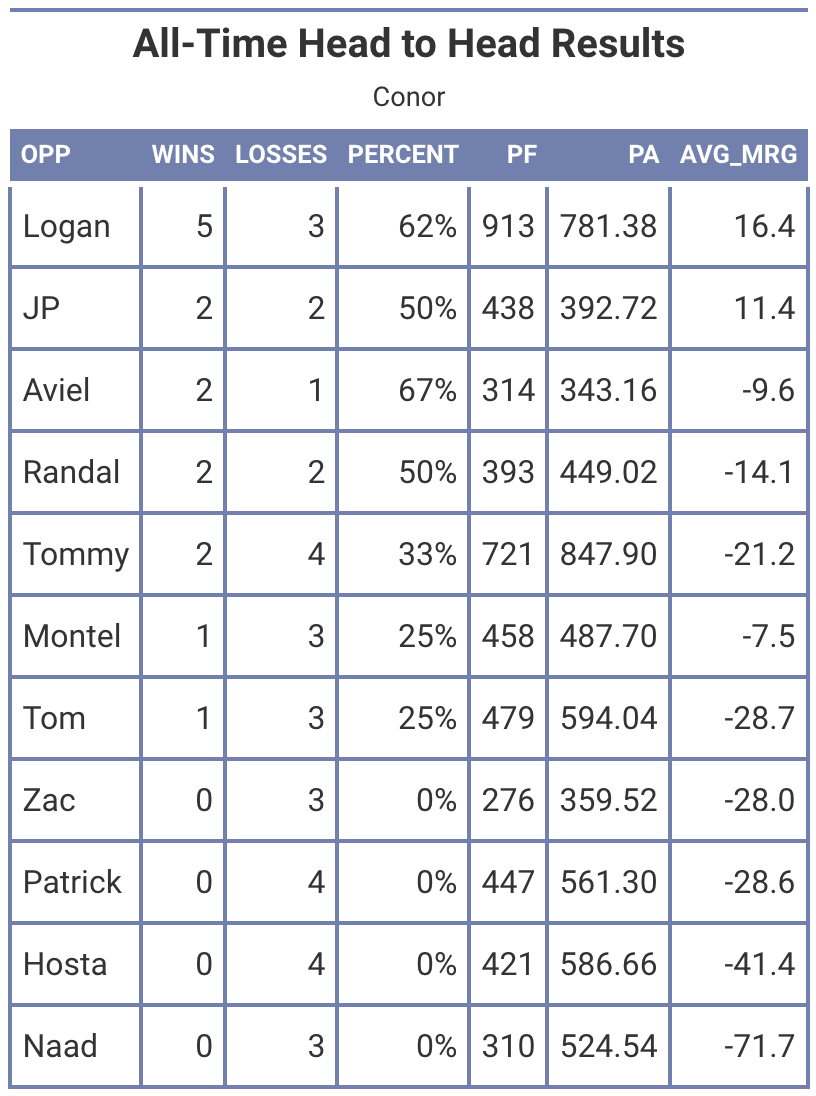
\includegraphics[width=0.48\linewidth,height=0.48\textheight]{output/headtohead/Conor_head_to_head} 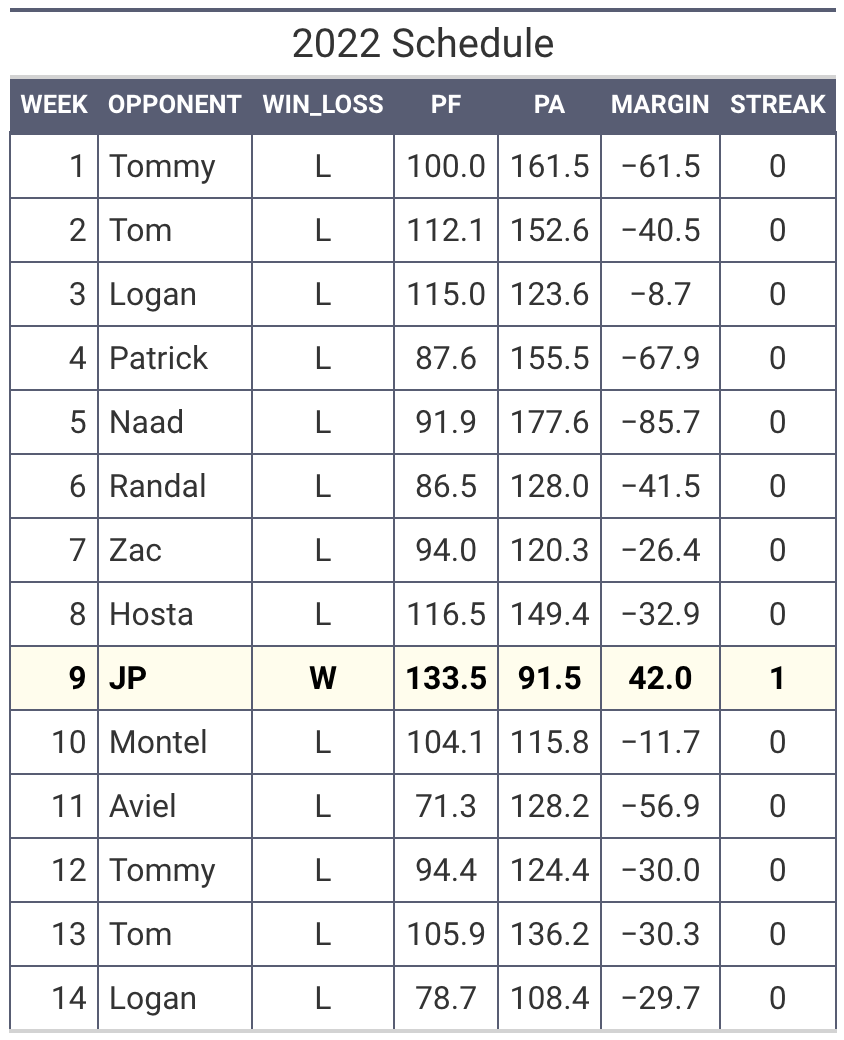
\includegraphics[width=0.48\linewidth,height=0.48\textheight]{output/py_schedule/season_results_Conor} 

}

\caption{The Outcomes}\label{fig:unnamed-chunk-20}
\end{figure}
\newpage

\hypertarget{el-randal}{%
\subsubsection{El Randal}\label{el-randal}}

\textbf{2023 Proj. \& 2022 Final Rosters}

\begin{figure}

{\centering \includegraphics[width=0.7\linewidth,height=0.7\textheight]{output/2023/dynasty_roster_Elrandal} \includegraphics[width=0.7\linewidth,height=0.7\textheight]{output/2022/dynasty_roster_Elrandal} 

}

\caption{The Ballers}\label{fig:unnamed-chunk-21}
\end{figure}
\newpage

\textbf{2022 Schedule \& Career Head to Head}

\begin{figure}

{\centering 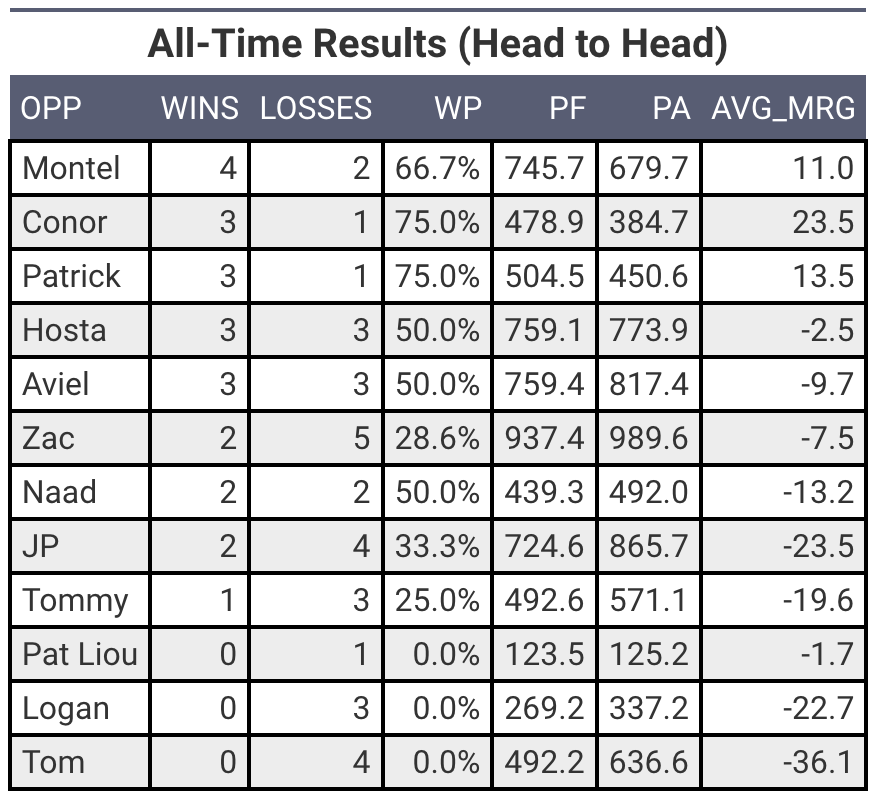
\includegraphics[width=0.48\linewidth,height=0.48\textheight]{output/headtohead/Randal_head_to_head} 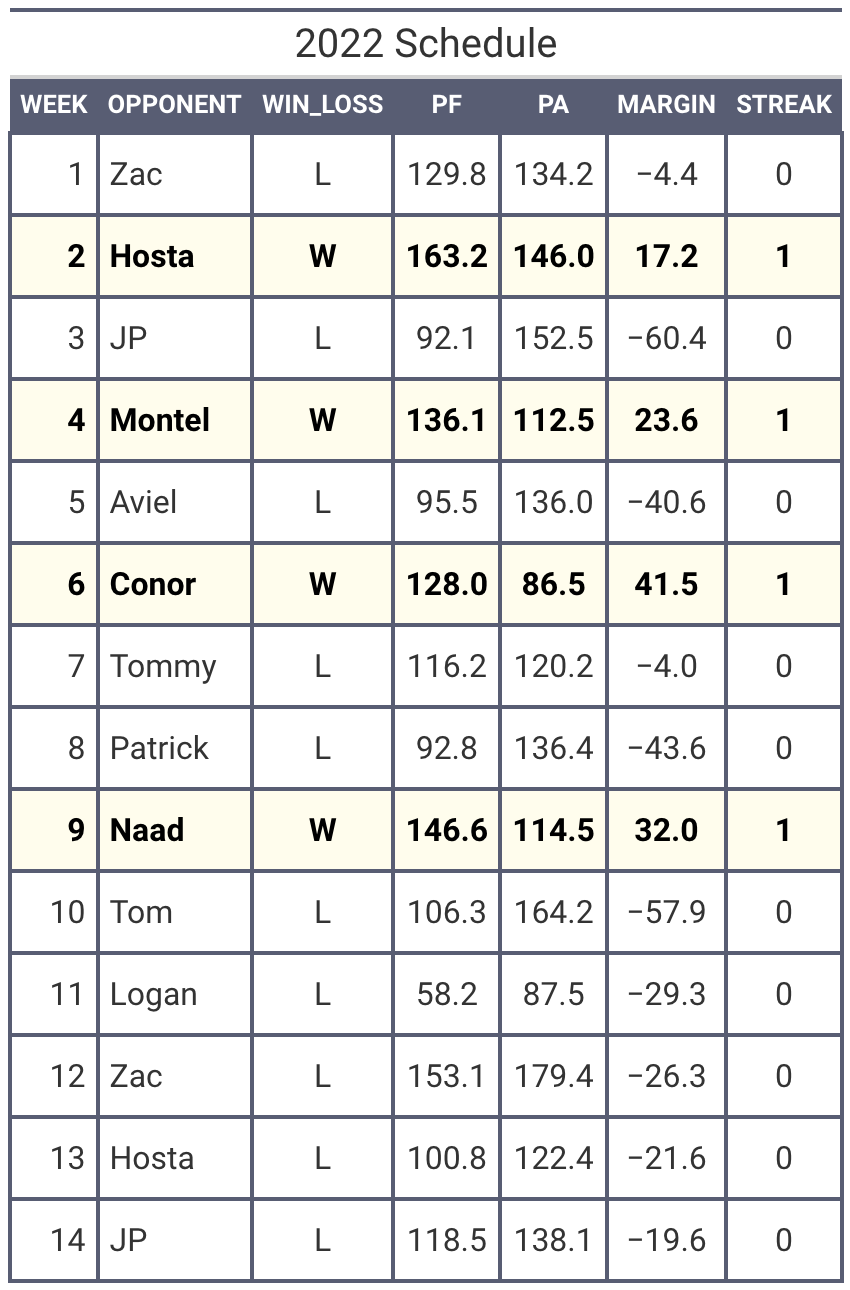
\includegraphics[width=0.48\linewidth,height=0.48\textheight]{output/py_schedule/season_results_Randal} 

}

\caption{The Outcomes}\label{fig:unnamed-chunk-22}
\end{figure}
\newpage

\hypertarget{general-t-sao-chicken}{%
\subsubsection{General T-sao Chicken}\label{general-t-sao-chicken}}

\textbf{2023 Proj. \& 2022 Final Rosters}

\begin{figure}

{\centering \includegraphics[width=0.7\linewidth,height=0.7\textheight]{output/2023/dynasty_roster_Ttsao} \includegraphics[width=0.7\linewidth,height=0.7\textheight]{output/2022/dynasty_roster_Ttsao} 

}

\caption{The Ballers}\label{fig:unnamed-chunk-23}
\end{figure}
\newpage

\textbf{2022 Schedule \& Career Head to Head}

\begin{figure}

{\centering 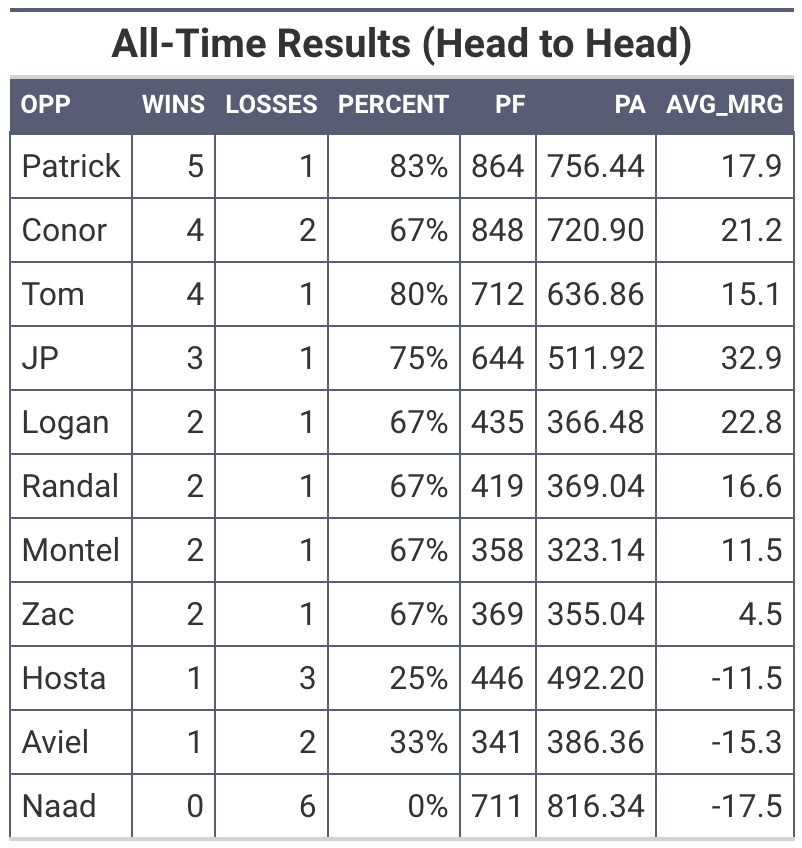
\includegraphics[width=0.48\linewidth,height=0.48\textheight]{output/headtohead/Tommy_head_to_head} 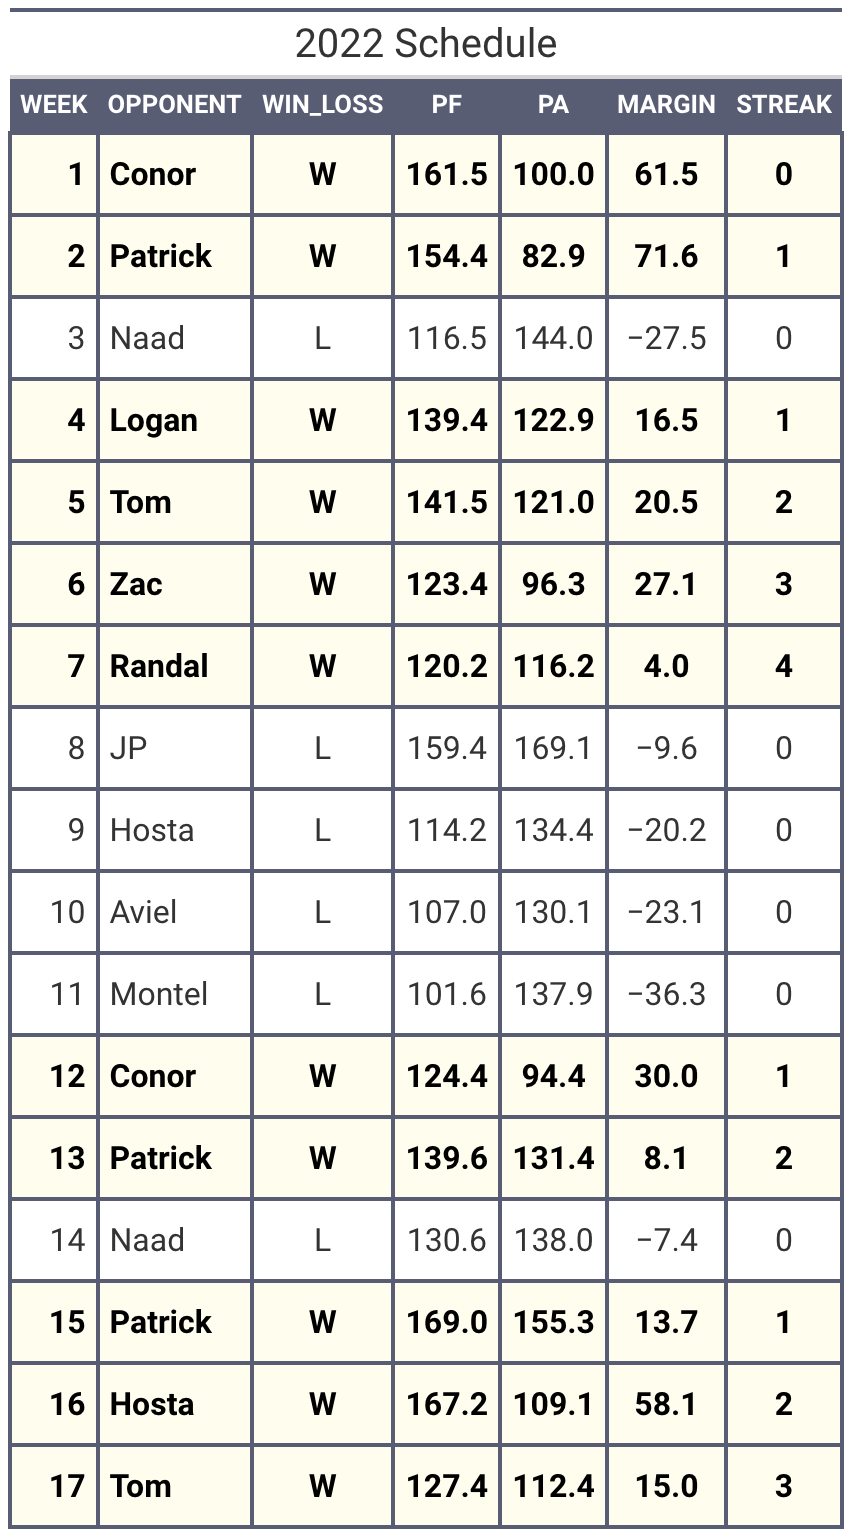
\includegraphics[width=0.48\linewidth,height=0.48\textheight]{output/py_schedule/season_results_Tommy} 

}

\caption{The Outcomes}\label{fig:unnamed-chunk-24}
\end{figure}

\hypertarget{pbpablo}{%
\subsubsection{pbpablo}\label{pbpablo}}

\textbf{2023 Proj. \& 2022 Final Rosters}

\begin{figure}

{\centering \includegraphics[width=0.7\linewidth,height=0.7\textheight]{output/2023/dynasty_roster_Pdpablo} \includegraphics[width=0.7\linewidth,height=0.7\textheight]{output/2022/dynasty_roster_Pdpablo} 

}

\caption{The Ballers}\label{fig:unnamed-chunk-25}
\end{figure}
\newpage

\textbf{2022 Schedule \& Career Head to Head}

\begin{figure}

{\centering \includegraphics[width=0.48\linewidth,height=0.48\textheight]{output/headtohead/Patrick_head_to_head} \includegraphics[width=0.48\linewidth,height=0.48\textheight]{output/py_schedule/season_results_Patrick} 

}

\caption{The Outcomes}\label{fig:unnamed-chunk-26}
\end{figure}

\hypertarget{slobonmynoblin-rip}{%
\subsubsection{slobonmynoblin (RIP)}\label{slobonmynoblin-rip}}

\textbf{2023 Proj. \& 2022 Final Rosters}

\begin{figure}

{\centering \includegraphics[width=0.7\linewidth,height=0.7\textheight]{output/2023/dynasty_roster_Slobonmynoblin} \includegraphics[width=0.7\linewidth,height=0.7\textheight]{output/2022/dynasty_roster_Slobonmynoblin} 

}

\caption{The Ballers}\label{fig:unnamed-chunk-27}
\end{figure}
\newpage

\textbf{2022 Schedule \& Career Head to Head}

\begin{figure}

{\centering \includegraphics[width=0.48\linewidth,height=0.48\textheight]{output/headtohead/Logan_head_to_head} \includegraphics[width=0.48\linewidth,height=0.48\textheight]{output/py_schedule/season_results_Logan} 

}

\caption{The Outcomes}\label{fig:unnamed-chunk-28}
\end{figure}

\end{document}
